\documentclass[twoside]{book}

% Packages required by doxygen
\usepackage{fixltx2e}
\usepackage{calc}
\usepackage{doxygen}
\usepackage[export]{adjustbox} % also loads graphicx
\usepackage{graphicx}
\usepackage[utf8]{inputenc}
\usepackage{makeidx}
\usepackage{multicol}
\usepackage{multirow}
\PassOptionsToPackage{warn}{textcomp}
\usepackage{textcomp}
\usepackage[nointegrals]{wasysym}
\usepackage[table]{xcolor}

% Font selection
\usepackage[T1]{fontenc}
\usepackage[scaled=.90]{helvet}
\usepackage{courier}
\usepackage{amssymb}
\usepackage{sectsty}
\renewcommand{\familydefault}{\sfdefault}
\allsectionsfont{%
  \fontseries{bc}\selectfont%
  \color{darkgray}%
}
\renewcommand{\DoxyLabelFont}{%
  \fontseries{bc}\selectfont%
  \color{darkgray}%
}
\newcommand{\+}{\discretionary{\mbox{\scriptsize$\hookleftarrow$}}{}{}}

% Page & text layout
\usepackage{geometry}
\geometry{%
  a4paper,%
  top=2.5cm,%
  bottom=2.5cm,%
  left=2.5cm,%
  right=2.5cm%
}
\tolerance=750
\hfuzz=15pt
\hbadness=750
\setlength{\emergencystretch}{15pt}
\setlength{\parindent}{0cm}
\setlength{\parskip}{3ex plus 2ex minus 2ex}
\makeatletter
\renewcommand{\paragraph}{%
  \@startsection{paragraph}{4}{0ex}{-1.0ex}{1.0ex}{%
    \normalfont\normalsize\bfseries\SS@parafont%
  }%
}
\renewcommand{\subparagraph}{%
  \@startsection{subparagraph}{5}{0ex}{-1.0ex}{1.0ex}{%
    \normalfont\normalsize\bfseries\SS@subparafont%
  }%
}
\makeatother

% Headers & footers
\usepackage{fancyhdr}
\pagestyle{fancyplain}
\fancyhead[LE]{\fancyplain{}{\bfseries\thepage}}
\fancyhead[CE]{\fancyplain{}{}}
\fancyhead[RE]{\fancyplain{}{\bfseries\leftmark}}
\fancyhead[LO]{\fancyplain{}{\bfseries\rightmark}}
\fancyhead[CO]{\fancyplain{}{}}
\fancyhead[RO]{\fancyplain{}{\bfseries\thepage}}
\fancyfoot[LE]{\fancyplain{}{}}
\fancyfoot[CE]{\fancyplain{}{}}
\fancyfoot[RE]{\fancyplain{}{\bfseries\scriptsize Generated by Doxygen }}
\fancyfoot[LO]{\fancyplain{}{\bfseries\scriptsize Generated by Doxygen }}
\fancyfoot[CO]{\fancyplain{}{}}
\fancyfoot[RO]{\fancyplain{}{}}
\renewcommand{\footrulewidth}{0.4pt}
\renewcommand{\chaptermark}[1]{%
  \markboth{#1}{}%
}
\renewcommand{\sectionmark}[1]{%
  \markright{\thesection\ #1}%
}

% Indices & bibliography
\usepackage{natbib}
\usepackage[titles]{tocloft}
\setcounter{tocdepth}{3}
\setcounter{secnumdepth}{5}
\makeindex

% Hyperlinks (required, but should be loaded last)
\usepackage{ifpdf}
\ifpdf
  \usepackage[pdftex,pagebackref=true]{hyperref}
\else
  \usepackage[ps2pdf,pagebackref=true]{hyperref}
\fi
\hypersetup{%
  colorlinks=true,%
  linkcolor=blue,%
  citecolor=blue,%
  unicode%
}

% Custom commands
\newcommand{\clearemptydoublepage}{%
  \newpage{\pagestyle{empty}\cleardoublepage}%
}

\usepackage{caption}
\captionsetup{labelsep=space,justification=centering,font={bf},singlelinecheck=off,skip=4pt,position=top}

%===== C O N T E N T S =====

\begin{document}

% Titlepage & ToC
\hypersetup{pageanchor=false,
             bookmarksnumbered=true,
             pdfencoding=unicode
            }
\pagenumbering{roman}
\begin{titlepage}
\vspace*{7cm}
\begin{center}%
{\Large Alarm Sytem }\\
\vspace*{1cm}
{\large Generated by Doxygen 1.8.11}\\
\end{center}
\end{titlepage}
\clearemptydoublepage
\tableofcontents
\clearemptydoublepage
\pagenumbering{arabic}
\hypersetup{pageanchor=true}

%--- Begin generated contents ---
\chapter{Alarm system}
\label{index}\hypertarget{index}{}\subsection*{Description}

This is the Alarm System implementation for Lab 2 of Media Processing course. Following diagram represents the model of the system divided into packages. Each package reprsesents separate module.

\subsubsection*{Main class diagram\+:}



\subsection*{Documentation}

Doxygen generated documentation is available in docs/html/index.\+html

\subsection*{Project structure}

\subsubsection*{Alarm\+Sensors}

Alarm\+Sensors group is located in {\ttfamily alarm-\/sensor} directory and includes sensor classes, i.\+e. {\ttfamily \hyperlink{classAbstractSensor}{Abstract\+Sensor}} class, which defines common attributes and operations and its different implementation, for instance, {\ttfamily \hyperlink{classSmokeSensor}{Smoke\+Sensor}} class. Whenever new sensor class is created it is sufficient that this class should be inherited from {\ttfamily \hyperlink{classAbstractSensor}{Abstract\+Sensor}} class, and {\ttfamily update()} function should be defined.

Here is the class diagram of Alarm\+Sensors package\+:



\subsubsection*{Alarm\+Composite}

Alarm\+Composite group is an implementation of composite pattern. It is located in {\ttfamily alarm-\/composite} directory. It includes base component class {\ttfamily \hyperlink{classAlarmComponent}{Alarm\+Component}} and its successor class {\ttfamily \hyperlink{classAlarmComponentGroup}{Alarm\+Component\+Group}}. Leaf implementation {\ttfamily \hyperlink{classAbstractSensor}{Abstract\+Sensor}} is a part of Alarm\+Sensors group.

Here is the class diagram of Alarm\+Composite package\+:



\subsubsection*{\hyperlink{classAlarmObserver}{Alarm\+Observer}}

\hyperlink{classAlarmObserver}{Alarm\+Observer} group is located in {\ttfamily alarm-\/observer}. It includes {\ttfamily \hyperlink{classAlarmObservable}{Alarm\+Observable}} class, which is a base for any actual implementation of observable objects. The only difference between Observer and Strategy here is that Observer can handle a message coming from observable, when Strategy can only be activated/deactivated by strategy owner. Observer is implemented in {\ttfamily \hyperlink{classAlarmObserver}{Alarm\+Observer}} class. In order to create new alarm strategy, one must inherit it from {\ttfamily \hyperlink{classAlarmObserver}{Alarm\+Observer}} base class and optionally redefine {\ttfamily handle function}.

Here is the class diagram of \hyperlink{classAlarmObserver}{Alarm\+Observer} package\+:



\subsubsection*{Alarm\+Strategies}

Alarm\+Strategies group is located in {\ttfamily alarm-\/strategy}. It includes {\ttfamily \hyperlink{classAlarmStrategy}{Alarm\+Strategy}} class, which is a base for any actual implementation of strategy. Context is implemented in {\ttfamily \hyperlink{classAlarmStrategyOwner}{Alarm\+Strategy\+Owner}} class. In order to create new alarm strategy, one must inherit it from {\ttfamily \hyperlink{classAlarmStrategy}{Alarm\+Strategy}} base class.

Here is the class diagram of Alarm\+Strategies package\+:



\subsection*{T\+O\+DO}


\begin{DoxyItemize}
\item \mbox{[}x\mbox{]} Implement Composite structure (classes \hyperlink{classAlarmComponent}{Alarm\+Component}, \hyperlink{classAlarmComponentGroup}{Alarm\+Component\+Group})
\item \mbox{[}x\mbox{]} Implement Strategy structure ( classes \hyperlink{classAlarmStrategy}{Alarm\+Strategy} and \hyperlink{classAlarmStrategyOwner}{Alarm\+Strategy\+Owner})
\item \mbox{[}x\mbox{]} Implement Alarm\+Sensor class
\item \mbox{[}x\mbox{]} Implement \hyperlink{classAlarmStrategy}{Alarm\+Strategy} successors
\item \mbox{[}x\mbox{]} Implement Alarm\+Sensor successors
\begin{DoxyItemize}
\item \mbox{[}x\mbox{]} Implement \hyperlink{classSmokeSensor}{Smoke\+Sensor}
\item \mbox{[}x\mbox{]} Implement \hyperlink{classMotionSensor}{Motion\+Sensor}
\item \mbox{[}x\mbox{]} Implement \hyperlink{classToxicSensor}{Toxic\+Sensor}
\end{DoxyItemize}
\item \mbox{[}x\mbox{]} Create documentation
\item \mbox{[}x\mbox{]} Reorganize project structure
\item \mbox{[}x\mbox{]} Implement operators
\begin{DoxyItemize}
\item \mbox{[}x\mbox{]} Implement operator++
\item \mbox{[}x\mbox{]} Implement operator-\/-\/
\item \mbox{[}x\mbox{]} Implement operator$<$$<$ for each type of sensor
\end{DoxyItemize}
\item \mbox{[}x\mbox{]} Add activation flag to \hyperlink{classAlarmComponent}{Alarm\+Component} and activation counter to \hyperlink{classAlarmStrategy}{Alarm\+Strategy}
\item \mbox{[}x\mbox{]} Parent attribute for \hyperlink{classAlarmComponent}{Alarm\+Component}
\item \mbox{[}x\mbox{]} Implement Observer structure
\item \mbox{[}x\mbox{]} Sorting and search algorithms
\item \mbox{[}x\mbox{]} Add model to the project
\item \mbox{[}x\mbox{]} Move sources to separate folder 
\end{DoxyItemize}
\chapter{Module Index}
\section{Modules}
Here is a list of all modules\+:\begin{DoxyCompactList}
\item \contentsline{section}{Alarm\+Composite}{\pageref{group__AlarmComposite}}{}
\item \contentsline{section}{Alarm\+Sensors}{\pageref{group__AlarmSensors}}{}
\item \contentsline{section}{Alarm\+Strategies}{\pageref{group__AlarmStrategies}}{}
\end{DoxyCompactList}

\chapter{Hierarchical Index}
\section{Class Hierarchy}
This inheritance list is sorted roughly, but not completely, alphabetically\+:\begin{DoxyCompactList}
\item \contentsline{section}{Alarm\+Component}{\pageref{classAlarmComponent}}{}
\begin{DoxyCompactList}
\item \contentsline{section}{Abstract\+Sensor}{\pageref{classAbstractSensor}}{}
\begin{DoxyCompactList}
\item \contentsline{section}{Motion\+Sensor}{\pageref{classMotionSensor}}{}
\item \contentsline{section}{Smoke\+Sensor}{\pageref{classSmokeSensor}}{}
\item \contentsline{section}{Toxic\+Sensor}{\pageref{classToxicSensor}}{}
\end{DoxyCompactList}
\item \contentsline{section}{Alarm\+Component\+Group}{\pageref{classAlarmComponentGroup}}{}
\end{DoxyCompactList}
\item \contentsline{section}{Alarm\+Strategy}{\pageref{classAlarmStrategy}}{}
\begin{DoxyCompactList}
\item \contentsline{section}{Call\+Firemen}{\pageref{classCallFiremen}}{}
\item \contentsline{section}{Call\+Police}{\pageref{classCallPolice}}{}
\end{DoxyCompactList}
\item \contentsline{section}{Alarm\+Strategy\+Owner}{\pageref{classAlarmStrategyOwner}}{}
\begin{DoxyCompactList}
\item \contentsline{section}{Abstract\+Sensor}{\pageref{classAbstractSensor}}{}
\end{DoxyCompactList}
\end{DoxyCompactList}

\chapter{Class Index}
\section{Class List}
Here are the classes, structs, unions and interfaces with brief descriptions\+:\begin{DoxyCompactList}
\item\contentsline{section}{\hyperlink{classAbstractSensor}{Abstract\+Sensor} \\*Abstract sensor class }{\pageref{classAbstractSensor}}{}
\item\contentsline{section}{\hyperlink{classAlarmComponent}{Alarm\+Component} \\*Base component class of composite structure }{\pageref{classAlarmComponent}}{}
\item\contentsline{section}{\hyperlink{classAlarmComponentGroup}{Alarm\+Component\+Group} \\*Group component class of composite structure }{\pageref{classAlarmComponentGroup}}{}
\item\contentsline{section}{\hyperlink{classAlarmStrategy}{Alarm\+Strategy} \\*Strategy class implementation of strategy pattern }{\pageref{classAlarmStrategy}}{}
\item\contentsline{section}{\hyperlink{classAlarmStrategyOwner}{Alarm\+Strategy\+Owner} \\*Context class implementation of strategy pattern }{\pageref{classAlarmStrategyOwner}}{}
\item\contentsline{section}{\hyperlink{classCallFiremen}{Call\+Firemen} \\*Call firemen strategy class }{\pageref{classCallFiremen}}{}
\item\contentsline{section}{\hyperlink{classCallPolice}{Call\+Police} \\*Call police strategy class }{\pageref{classCallPolice}}{}
\item\contentsline{section}{\hyperlink{classMotionSensor}{Motion\+Sensor} \\*Motion sensor class }{\pageref{classMotionSensor}}{}
\item\contentsline{section}{\hyperlink{classSmokeSensor}{Smoke\+Sensor} \\*Smoke sensor class }{\pageref{classSmokeSensor}}{}
\item\contentsline{section}{\hyperlink{classToxicSensor}{Toxic\+Sensor} \\*Toxic sensor class }{\pageref{classToxicSensor}}{}
\end{DoxyCompactList}

\chapter{File Index}
\section{File List}
Here is a list of all documented files with brief descriptions\+:\begin{DoxyCompactList}
\item\contentsline{section}{alarm-\/composite/\hyperlink{alarmcomponent_8h}{alarmcomponent.\+h} }{\pageref{alarmcomponent_8h}}{}
\item\contentsline{section}{alarm-\/composite/\hyperlink{alarmcomponentgroup_8h}{alarmcomponentgroup.\+h} }{\pageref{alarmcomponentgroup_8h}}{}
\item\contentsline{section}{alarm-\/sensor/\hyperlink{abstractsensor_8h}{abstractsensor.\+h} }{\pageref{abstractsensor_8h}}{}
\item\contentsline{section}{alarm-\/sensor/\hyperlink{motionsensor_8h}{motionsensor.\+h} }{\pageref{motionsensor_8h}}{}
\item\contentsline{section}{alarm-\/sensor/\hyperlink{smokesensor_8h}{smokesensor.\+h} }{\pageref{smokesensor_8h}}{}
\item\contentsline{section}{alarm-\/sensor/\hyperlink{toxicsensor_8h}{toxicsensor.\+h} }{\pageref{toxicsensor_8h}}{}
\item\contentsline{section}{alarm-\/strategy/\hyperlink{alarmstrategy_8h}{alarmstrategy.\+h} }{\pageref{alarmstrategy_8h}}{}
\item\contentsline{section}{alarm-\/strategy/\hyperlink{alarmstrategyowner_8h}{alarmstrategyowner.\+h} }{\pageref{alarmstrategyowner_8h}}{}
\item\contentsline{section}{alarm-\/strategy/\hyperlink{callfiremen_8h}{callfiremen.\+h} }{\pageref{callfiremen_8h}}{}
\item\contentsline{section}{alarm-\/strategy/\hyperlink{callpolice_8h}{callpolice.\+h} }{\pageref{callpolice_8h}}{}
\end{DoxyCompactList}

\chapter{Module Documentation}
\hypertarget{group__AlarmComposite}{}\section{Alarm\+Composite}
\label{group__AlarmComposite}\index{Alarm\+Composite@{Alarm\+Composite}}


Composite pattern implementation.  


Collaboration diagram for Alarm\+Composite\+:\nopagebreak
\begin{figure}[H]
\begin{center}
\leavevmode
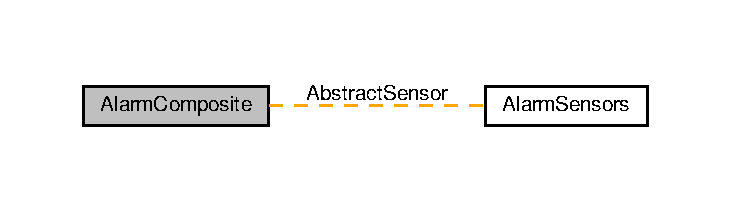
\includegraphics[width=350pt]{group__AlarmComposite}
\end{center}
\end{figure}
\subsection*{Classes}
\begin{DoxyCompactItemize}
\item 
class \hyperlink{classAlarmComponent}{Alarm\+Component}
\begin{DoxyCompactList}\small\item\em Base component class of composite structure. \end{DoxyCompactList}\item 
class \hyperlink{classAlarmComponentGroup}{Alarm\+Component\+Group}
\begin{DoxyCompactList}\small\item\em Group component class of composite structure. \end{DoxyCompactList}\item 
class \hyperlink{classAbstractSensor}{Abstract\+Sensor}
\begin{DoxyCompactList}\small\item\em Abstract sensor class. \end{DoxyCompactList}\end{DoxyCompactItemize}


\subsection{Detailed Description}
Composite pattern implementation. 

Includes base class \hyperlink{classAlarmComponent}{Alarm\+Component}, leaf class \hyperlink{classAbstractSensor}{Abstract\+Sensor}, and group class Abstract\+Component\+Group 
\hypertarget{group__AlarmObservation}{}\section{Alarm\+Observation}
\label{group__AlarmObservation}\index{Alarm\+Observation@{Alarm\+Observation}}


Observer pattern implementation.  


\subsection*{Classes}
\begin{DoxyCompactItemize}
\item 
class \hyperlink{classAlarmObservable}{Alarm\+Observable}
\begin{DoxyCompactList}\small\item\em Observable class of observer structure. \end{DoxyCompactList}\item 
class \hyperlink{classAlarmObserver}{Alarm\+Observer}
\begin{DoxyCompactList}\small\item\em Observer class of observer structure. \end{DoxyCompactList}\end{DoxyCompactItemize}


\subsection{Detailed Description}
Observer pattern implementation. 

Includes observable class \hyperlink{classAlarmObservable}{Alarm\+Observable}, which is inherited by \hyperlink{classAlarmComponent}{Alarm\+Component} and observer class \hyperlink{classAlarmObserver}{Alarm\+Observer} which should be inherited by any alarm observer imlementation 
\hypertarget{group__AlarmSensors}{}\section{Alarm\+Sensors}
\label{group__AlarmSensors}\index{Alarm\+Sensors@{Alarm\+Sensors}}


Sensors used in the system.  


Collaboration diagram for Alarm\+Sensors\+:\nopagebreak
\begin{figure}[H]
\begin{center}
\leavevmode
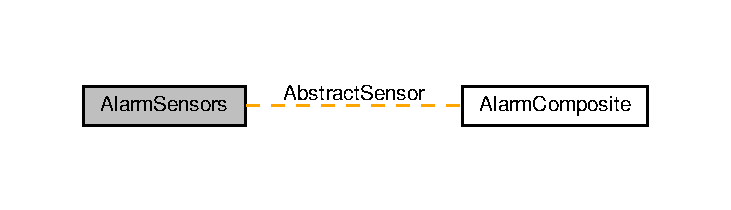
\includegraphics[width=350pt]{group__AlarmSensors}
\end{center}
\end{figure}
\subsection*{Classes}
\begin{DoxyCompactItemize}
\item 
class \hyperlink{classAbstractSensor}{Abstract\+Sensor}
\begin{DoxyCompactList}\small\item\em Abstract sensor class. \end{DoxyCompactList}\item 
class \hyperlink{classMotionSensor}{Motion\+Sensor}
\begin{DoxyCompactList}\small\item\em Motion sensor class. \end{DoxyCompactList}\item 
class \hyperlink{classSmokeSensor}{Smoke\+Sensor}
\begin{DoxyCompactList}\small\item\em Smoke sensor class. \end{DoxyCompactList}\item 
class \hyperlink{classToxicSensor}{Toxic\+Sensor}
\begin{DoxyCompactList}\small\item\em Toxic sensor class Dummy implementation of toxic sensor component. Intended for testing purposes. \end{DoxyCompactList}\end{DoxyCompactItemize}


\subsection{Detailed Description}
Sensors used in the system. 

Includes common predeccessor class \hyperlink{classAbstractSensor}{Abstract\+Sensor} and its successors.

\begin{DoxyNote}{Note}
In order to add sensor to the application, one needs to inherit a new sensor class from \hyperlink{classAbstractSensor}{Abstract\+Sensor} 
\end{DoxyNote}

\hypertarget{group__AlarmStrategies}{}\section{Alarm\+Strategies}
\label{group__AlarmStrategies}\index{Alarm\+Strategies@{Alarm\+Strategies}}


Strategy pattern implementation.  


\subsection*{Classes}
\begin{DoxyCompactItemize}
\item 
class \hyperlink{classAlarmStrategy}{Alarm\+Strategy}
\begin{DoxyCompactList}\small\item\em Strategy class implementation of strategy pattern. \end{DoxyCompactList}\item 
class \hyperlink{classAlarmStrategyOwner}{Alarm\+Strategy\+Owner}
\begin{DoxyCompactList}\small\item\em Context class implementation of strategy pattern. \end{DoxyCompactList}\item 
class \hyperlink{classCallFiremen}{Call\+Firemen}
\begin{DoxyCompactList}\small\item\em Call firemen strategy class. \end{DoxyCompactList}\item 
class \hyperlink{classCallPolice}{Call\+Police}
\begin{DoxyCompactList}\small\item\em Call police strategy class. \end{DoxyCompactList}\end{DoxyCompactItemize}


\subsection{Detailed Description}
Strategy pattern implementation. 


\chapter{Class Documentation}
\hypertarget{classAbstractSensor}{}\section{Abstract\+Sensor Class Reference}
\label{classAbstractSensor}\index{Abstract\+Sensor@{Abstract\+Sensor}}


Abstract sensor class.  




{\ttfamily \#include $<$abstractsensor.\+h$>$}



Inheritance diagram for Abstract\+Sensor\+:
\nopagebreak
\begin{figure}[H]
\begin{center}
\leavevmode
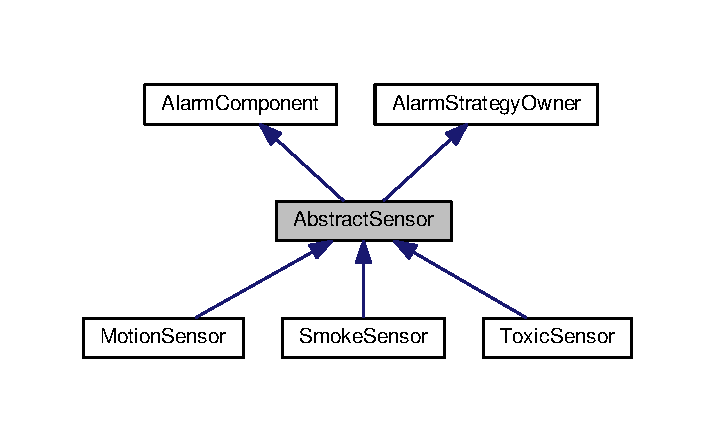
\includegraphics[width=346pt]{classAbstractSensor__inherit__graph}
\end{center}
\end{figure}


Collaboration diagram for Abstract\+Sensor\+:
\nopagebreak
\begin{figure}[H]
\begin{center}
\leavevmode
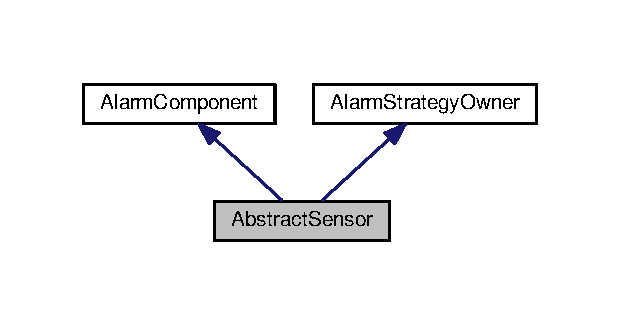
\includegraphics[width=350pt]{classAbstractSensor__coll__graph}
\end{center}
\end{figure}
\subsection*{Public Member Functions}
\begin{DoxyCompactItemize}
\item 
\hyperlink{classAbstractSensor_a6ce9232e9b428879bcdee6591eba55e6}{Abstract\+Sensor} (std\+::string id=\char`\"{}Unknown id\char`\"{}, std\+::string type=\char`\"{}Unknown type\char`\"{}, std\+::string vendor=\char`\"{}Unknown vendor\char`\"{})
\begin{DoxyCompactList}\small\item\em Class constructor. \end{DoxyCompactList}\item 
virtual void \hyperlink{classAbstractSensor_a8d0a1908c6aaf67fc7d781e54b49293b}{update} ()=0\hypertarget{classAbstractSensor_a8d0a1908c6aaf67fc7d781e54b49293b}{}\label{classAbstractSensor_a8d0a1908c6aaf67fc7d781e54b49293b}

\begin{DoxyCompactList}\small\item\em Pure virtual function to be defined in implementation class. \end{DoxyCompactList}\item 
virtual void \hyperlink{classAbstractSensor_a0071c6499b1538713bb46d07f0b30ca1}{activate} ()\hypertarget{classAbstractSensor_a0071c6499b1538713bb46d07f0b30ca1}{}\label{classAbstractSensor_a0071c6499b1538713bb46d07f0b30ca1}

\begin{DoxyCompactList}\small\item\em Activates the sensor, i.\+e. activates alarm strategies. \end{DoxyCompactList}\item 
virtual void \hyperlink{classAbstractSensor_a7f921f96118605def806c40139f5496b}{deactivate} ()\hypertarget{classAbstractSensor_a7f921f96118605def806c40139f5496b}{}\label{classAbstractSensor_a7f921f96118605def806c40139f5496b}

\begin{DoxyCompactList}\small\item\em Deactivates the sensor, i.\+e. deactivates alarm strategies. \end{DoxyCompactList}\item 
std\+::string \hyperlink{classAbstractSensor_a2786a5387ea8a90f8451cb3a64a3e152}{get\+Vendor} () const \hypertarget{classAbstractSensor_a2786a5387ea8a90f8451cb3a64a3e152}{}\label{classAbstractSensor_a2786a5387ea8a90f8451cb3a64a3e152}

\begin{DoxyCompactList}\small\item\em Returns vendor name. \end{DoxyCompactList}\item 
const std\+::string \hyperlink{classAbstractSensor_a31f55a2259b24f124b64a3ddd3004d6e}{get\+Type} () const \hypertarget{classAbstractSensor_a31f55a2259b24f124b64a3ddd3004d6e}{}\label{classAbstractSensor_a31f55a2259b24f124b64a3ddd3004d6e}

\begin{DoxyCompactList}\small\item\em Returns type of sensor. \end{DoxyCompactList}\item 
virtual const std\+::string \hyperlink{classAbstractSensor_a3b498785d810c29b3d20254a365adb43}{get\+Info} () const \hypertarget{classAbstractSensor_a3b498785d810c29b3d20254a365adb43}{}\label{classAbstractSensor_a3b498785d810c29b3d20254a365adb43}

\begin{DoxyCompactList}\small\item\em String stream containing info about the sensor. \end{DoxyCompactList}\end{DoxyCompactItemize}
\subsection*{Additional Inherited Members}


\subsection{Detailed Description}
Abstract sensor class. 

Defines common operations for alarm sensors

\begin{DoxyNote}{Note}
When inheriting from \hyperlink{classAbstractSensor}{Abstract\+Sensor}, one needs to redefine pure virtual method \hyperlink{classAbstractSensor_a8d0a1908c6aaf67fc7d781e54b49293b}{update()} 
\end{DoxyNote}


\subsection{Constructor \& Destructor Documentation}
\index{Abstract\+Sensor@{Abstract\+Sensor}!Abstract\+Sensor@{Abstract\+Sensor}}
\index{Abstract\+Sensor@{Abstract\+Sensor}!Abstract\+Sensor@{Abstract\+Sensor}}
\subsubsection[{\texorpdfstring{Abstract\+Sensor(std\+::string id=""Unknown id"", std\+::string type=""Unknown type"", std\+::string vendor=""Unknown vendor"")}{AbstractSensor(std::string id="Unknown id", std::string type="Unknown type", std::string vendor="Unknown vendor")}}]{\setlength{\rightskip}{0pt plus 5cm}Abstract\+Sensor\+::\+Abstract\+Sensor (
\begin{DoxyParamCaption}
\item[{std\+::string}]{id = {\ttfamily \char`\"{}Unknown~id\char`\"{}}, }
\item[{std\+::string}]{type = {\ttfamily \char`\"{}Unknown~type\char`\"{}}, }
\item[{std\+::string}]{vendor = {\ttfamily \char`\"{}Unknown~vendor\char`\"{}}}
\end{DoxyParamCaption}
)\hspace{0.3cm}{\ttfamily [explicit]}}\hypertarget{classAbstractSensor_a6ce9232e9b428879bcdee6591eba55e6}{}\label{classAbstractSensor_a6ce9232e9b428879bcdee6591eba55e6}


Class constructor. 


\begin{DoxyParams}{Parameters}
{\em id} & identificator of the sensor \\
\hline
{\em type} & type of the sensor \\
\hline
{\em vendor} & vendor name \\
\hline
\end{DoxyParams}


The documentation for this class was generated from the following files\+:\begin{DoxyCompactItemize}
\item 
alarm-\/sensor/\hyperlink{abstractsensor_8h}{abstractsensor.\+h}\item 
alarm-\/sensor/abstractsensor.\+cpp\end{DoxyCompactItemize}

\hypertarget{classAlarmComponent}{}\section{Alarm\+Component Class Reference}
\label{classAlarmComponent}\index{Alarm\+Component@{Alarm\+Component}}


Base component class of composite structure.  




{\ttfamily \#include $<$alarmcomponent.\+h$>$}



Inheritance diagram for Alarm\+Component\+:\nopagebreak
\begin{figure}[H]
\begin{center}
\leavevmode
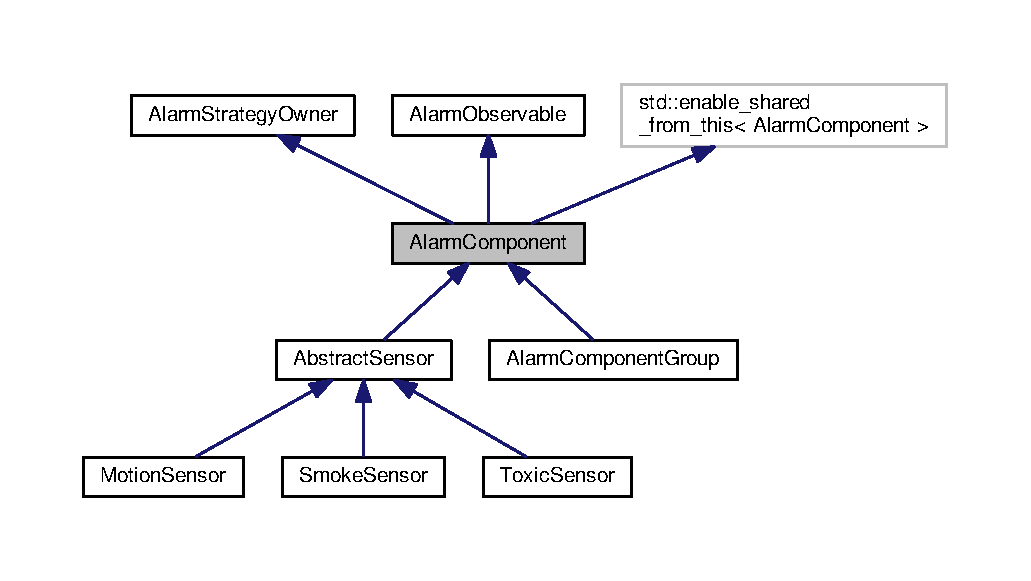
\includegraphics[width=350pt]{classAlarmComponent__inherit__graph}
\end{center}
\end{figure}


Collaboration diagram for Alarm\+Component\+:\nopagebreak
\begin{figure}[H]
\begin{center}
\leavevmode
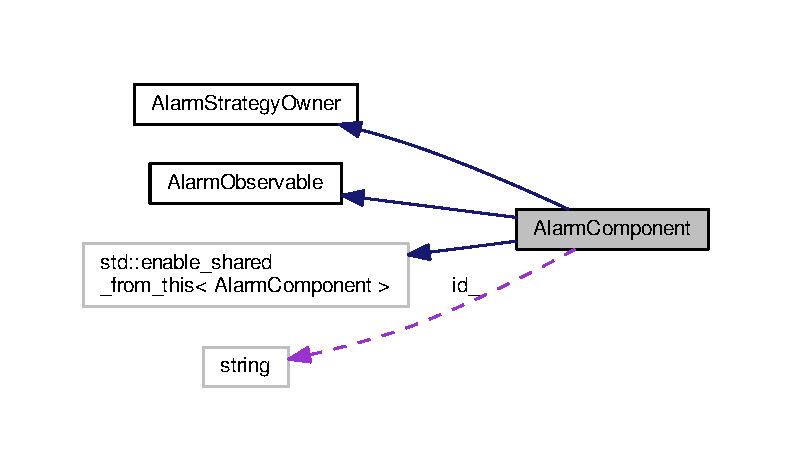
\includegraphics[width=350pt]{classAlarmComponent__coll__graph}
\end{center}
\end{figure}
\subsection*{Public Types}
\begin{DoxyCompactItemize}
\item 
typedef std\+::shared\+\_\+ptr$<$ \hyperlink{classAlarmComponent}{Alarm\+Component} $>$ {\bfseries S\+Ptr}\hypertarget{classAlarmComponent_a508e811a15269806af1a18aa4d387128}{}\label{classAlarmComponent_a508e811a15269806af1a18aa4d387128}

\end{DoxyCompactItemize}
\subsection*{Public Member Functions}
\begin{DoxyCompactItemize}
\item 
\hyperlink{classAlarmComponent_a7e726c4fb79d226772182fe979967028}{Alarm\+Component} (const std\+::string \&id)
\begin{DoxyCompactList}\small\item\em Class constructor. \end{DoxyCompactList}\item 
virtual void \hyperlink{classAlarmComponent_ab2acf6b580efe04bd617580ecb7323f1}{activate} ()\hypertarget{classAlarmComponent_ab2acf6b580efe04bd617580ecb7323f1}{}\label{classAlarmComponent_ab2acf6b580efe04bd617580ecb7323f1}

\begin{DoxyCompactList}\small\item\em Activation of the component. \end{DoxyCompactList}\item 
virtual void \hyperlink{classAlarmComponent_aef44069a068e92ccd15b3afcbd06dff6}{deactivate} ()\hypertarget{classAlarmComponent_aef44069a068e92ccd15b3afcbd06dff6}{}\label{classAlarmComponent_aef44069a068e92ccd15b3afcbd06dff6}

\begin{DoxyCompactList}\small\item\em Deactivation of the component. \end{DoxyCompactList}\item 
virtual void \hyperlink{classAlarmComponent_a51a7a6e0d85da344c741deddfcb7cff3}{print\+Info} ()\hypertarget{classAlarmComponent_a51a7a6e0d85da344c741deddfcb7cff3}{}\label{classAlarmComponent_a51a7a6e0d85da344c741deddfcb7cff3}

\begin{DoxyCompactList}\small\item\em Print component info. \end{DoxyCompactList}\item 
const std\+::string \& \hyperlink{classAlarmComponent_a7d576b833767677aef88ac0e53dc5f22}{get\+Id} () const \hypertarget{classAlarmComponent_a7d576b833767677aef88ac0e53dc5f22}{}\label{classAlarmComponent_a7d576b833767677aef88ac0e53dc5f22}

\begin{DoxyCompactList}\small\item\em Returns id of the component. \end{DoxyCompactList}\item 
const S\+Ptr \hyperlink{classAlarmComponent_ab105241dfaade407b9683bb32e8d0f2f}{get\+Root\+Component} ()
\begin{DoxyCompactList}\small\item\em Get root object of the group. \end{DoxyCompactList}\item 
void \hyperlink{classAlarmComponent_a8a23397273077d5808735d083878378a}{set\+Parent} (const S\+Ptr \&sptr)
\begin{DoxyCompactList}\small\item\em Set the parent of the component. \end{DoxyCompactList}\item 
const bool \& \hyperlink{classAlarmComponent_ad445ad4870607e5305ef6e7eee10eb3b}{is\+Activated} ()\hypertarget{classAlarmComponent_ad445ad4870607e5305ef6e7eee10eb3b}{}\label{classAlarmComponent_ad445ad4870607e5305ef6e7eee10eb3b}

\begin{DoxyCompactList}\small\item\em Read activation status. \end{DoxyCompactList}\item 
virtual void \hyperlink{classAlarmComponent_ae94d389ca9933e31e2bda486eb5b7c1f}{notify} (const std\+::string msg) override
\begin{DoxyCompactList}\small\item\em Notify observers. \end{DoxyCompactList}\end{DoxyCompactItemize}
\subsection*{Protected Attributes}
\begin{DoxyCompactItemize}
\item 
std\+::string \hyperlink{classAlarmComponent_aad0807ccc068a68b5cc43bf307689069}{id\+\_\+}\hypertarget{classAlarmComponent_aad0807ccc068a68b5cc43bf307689069}{}\label{classAlarmComponent_aad0807ccc068a68b5cc43bf307689069}

\begin{DoxyCompactList}\small\item\em identificator of the component \end{DoxyCompactList}\item 
S\+Ptr \hyperlink{classAlarmComponent_a6d7ef82bfe60f4d31e5f340139ccff1b}{parent\+\_\+}\hypertarget{classAlarmComponent_a6d7ef82bfe60f4d31e5f340139ccff1b}{}\label{classAlarmComponent_a6d7ef82bfe60f4d31e5f340139ccff1b}

\begin{DoxyCompactList}\small\item\em parent of the component \end{DoxyCompactList}\item 
bool \hyperlink{classAlarmComponent_a187ca6cd2f8310b5be8000c58934a746}{activated\+\_\+}\hypertarget{classAlarmComponent_a187ca6cd2f8310b5be8000c58934a746}{}\label{classAlarmComponent_a187ca6cd2f8310b5be8000c58934a746}

\begin{DoxyCompactList}\small\item\em activation flag \end{DoxyCompactList}\end{DoxyCompactItemize}


\subsection{Detailed Description}
Base component class of composite structure. 

\subsection{Constructor \& Destructor Documentation}
\index{Alarm\+Component@{Alarm\+Component}!Alarm\+Component@{Alarm\+Component}}
\index{Alarm\+Component@{Alarm\+Component}!Alarm\+Component@{Alarm\+Component}}
\subsubsection[{\texorpdfstring{Alarm\+Component(const std\+::string \&id)}{AlarmComponent(const std::string &id)}}]{\setlength{\rightskip}{0pt plus 5cm}Alarm\+Component\+::\+Alarm\+Component (
\begin{DoxyParamCaption}
\item[{const std\+::string \&}]{id}
\end{DoxyParamCaption}
)\hspace{0.3cm}{\ttfamily [explicit]}}\hypertarget{classAlarmComponent_a7e726c4fb79d226772182fe979967028}{}\label{classAlarmComponent_a7e726c4fb79d226772182fe979967028}


Class constructor. 


\begin{DoxyParams}{Parameters}
{\em id} & identificator of the component \\
\hline
\end{DoxyParams}


\subsection{Member Function Documentation}
\index{Alarm\+Component@{Alarm\+Component}!get\+Root\+Component@{get\+Root\+Component}}
\index{get\+Root\+Component@{get\+Root\+Component}!Alarm\+Component@{Alarm\+Component}}
\subsubsection[{\texorpdfstring{get\+Root\+Component()}{getRootComponent()}}]{\setlength{\rightskip}{0pt plus 5cm}const Alarm\+Component\+::\+S\+Ptr Alarm\+Component\+::get\+Root\+Component (
\begin{DoxyParamCaption}
{}
\end{DoxyParamCaption}
)}\hypertarget{classAlarmComponent_ab105241dfaade407b9683bb32e8d0f2f}{}\label{classAlarmComponent_ab105241dfaade407b9683bb32e8d0f2f}


Get root object of the group. 

Return root object of a group component is in or component itself if a component is a root object \index{Alarm\+Component@{Alarm\+Component}!notify@{notify}}
\index{notify@{notify}!Alarm\+Component@{Alarm\+Component}}
\subsubsection[{\texorpdfstring{notify(const std\+::string msg) override}{notify(const std::string msg) override}}]{\setlength{\rightskip}{0pt plus 5cm}void Alarm\+Component\+::notify (
\begin{DoxyParamCaption}
\item[{const std\+::string}]{msg}
\end{DoxyParamCaption}
)\hspace{0.3cm}{\ttfamily [override]}, {\ttfamily [virtual]}}\hypertarget{classAlarmComponent_ae94d389ca9933e31e2bda486eb5b7c1f}{}\label{classAlarmComponent_ae94d389ca9933e31e2bda486eb5b7c1f}


Notify observers. 

Notifies observers and passes notification to the parent.

\begin{DoxyNote}{Note}
this is an overloaded function of \hyperlink{classAlarmObservable_afe90d2612d363050a620eb8b2ef2fa0a}{Alarm\+Observable\+::notify} 
\end{DoxyNote}


Reimplemented from \hyperlink{classAlarmObservable_afe90d2612d363050a620eb8b2ef2fa0a}{Alarm\+Observable}.

\index{Alarm\+Component@{Alarm\+Component}!set\+Parent@{set\+Parent}}
\index{set\+Parent@{set\+Parent}!Alarm\+Component@{Alarm\+Component}}
\subsubsection[{\texorpdfstring{set\+Parent(const S\+Ptr \&sptr)}{setParent(const SPtr &sptr)}}]{\setlength{\rightskip}{0pt plus 5cm}void Alarm\+Component\+::set\+Parent (
\begin{DoxyParamCaption}
\item[{const S\+Ptr \&}]{sptr}
\end{DoxyParamCaption}
)}\hypertarget{classAlarmComponent_a8a23397273077d5808735d083878378a}{}\label{classAlarmComponent_a8a23397273077d5808735d083878378a}


Set the parent of the component. 


\begin{DoxyParams}{Parameters}
{\em sptr} & parent \\
\hline
\end{DoxyParams}


The documentation for this class was generated from the following files\+:\begin{DoxyCompactItemize}
\item 
alarm-\/composite/\hyperlink{alarmcomponent_8h}{alarmcomponent.\+h}\item 
alarm-\/composite/\hyperlink{alarmcomponent_8cpp}{alarmcomponent.\+cpp}\end{DoxyCompactItemize}

\hypertarget{classAlarmComponentGroup}{}\section{Alarm\+Component\+Group Class Reference}
\label{classAlarmComponentGroup}\index{Alarm\+Component\+Group@{Alarm\+Component\+Group}}


Group component class of composite structure.  




{\ttfamily \#include $<$alarmcomponentgroup.\+h$>$}



Inheritance diagram for Alarm\+Component\+Group\+:\nopagebreak
\begin{figure}[H]
\begin{center}
\leavevmode
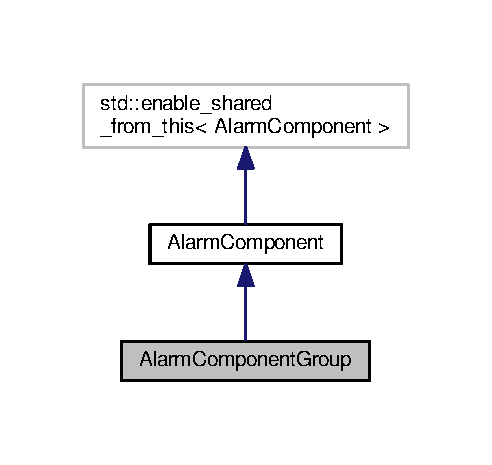
\includegraphics[width=346pt]{classAlarmComponentGroup__inherit__graph}
\end{center}
\end{figure}


Collaboration diagram for Alarm\+Component\+Group\+:\nopagebreak
\begin{figure}[H]
\begin{center}
\leavevmode
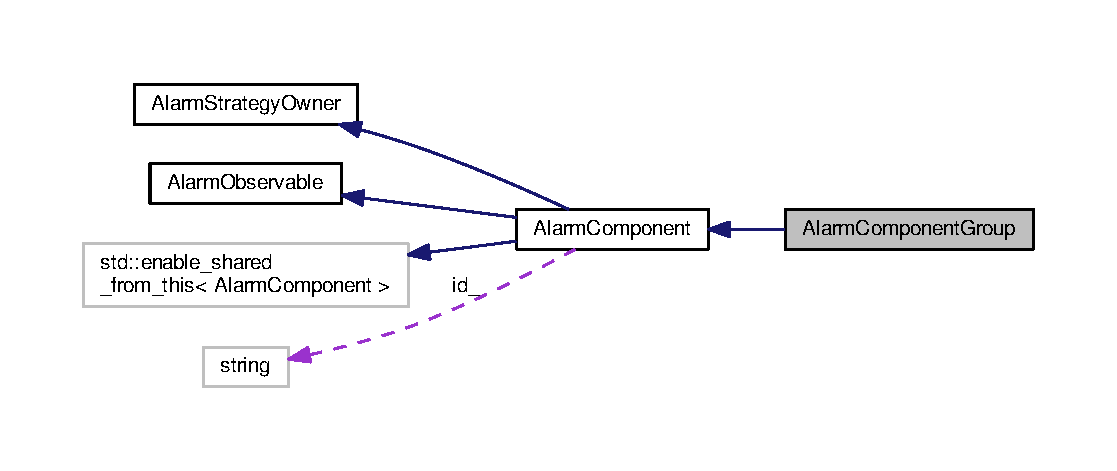
\includegraphics[width=350pt]{classAlarmComponentGroup__coll__graph}
\end{center}
\end{figure}
\subsection*{Public Member Functions}
\begin{DoxyCompactItemize}
\item 
\hyperlink{classAlarmComponentGroup_af999ab1dac77f573df01fb400ec5d044}{Alarm\+Component\+Group} (std\+::string id=\char`\"{}unknown group\char`\"{})
\begin{DoxyCompactList}\small\item\em Class constructor. \end{DoxyCompactList}\item 
virtual void \hyperlink{classAlarmComponentGroup_ac67076993e9068dc15e8d39af29698a4}{activate} () finaloverride
\begin{DoxyCompactList}\small\item\em Activation of the component group. \end{DoxyCompactList}\item 
virtual void \hyperlink{classAlarmComponentGroup_a673cebdc7e32c522af0e7435786ea118}{deactivate} () finaloverride
\begin{DoxyCompactList}\small\item\em Dectivation of the component group. \end{DoxyCompactList}\item 
virtual void \hyperlink{classAlarmComponentGroup_a76c37915b10d54349ebf246fddbc603a}{print\+Info} () const override\hypertarget{classAlarmComponentGroup_a76c37915b10d54349ebf246fddbc603a}{}\label{classAlarmComponentGroup_a76c37915b10d54349ebf246fddbc603a}

\begin{DoxyCompactList}\small\item\em Print info about the group Print info about the group, including info about each component inside the group. \end{DoxyCompactList}\item 
void \hyperlink{classAlarmComponentGroup_ac07c12720297df1bbf1e131af6631049}{add} (const Alarm\+Component\+::\+S\+Ptr \&sptr)
\begin{DoxyCompactList}\small\item\em Add component to the group. \end{DoxyCompactList}\item 
void \hyperlink{classAlarmComponentGroup_a4e6c27c533e73d95fe622ca8ed89a9ae}{remove} (const Alarm\+Component\+::\+S\+Ptr \&sptr)
\begin{DoxyCompactList}\small\item\em Remove component from the group. \end{DoxyCompactList}\end{DoxyCompactItemize}
\subsection*{Additional Inherited Members}


\subsection{Detailed Description}
Group component class of composite structure. 

\subsection{Constructor \& Destructor Documentation}
\index{Alarm\+Component\+Group@{Alarm\+Component\+Group}!Alarm\+Component\+Group@{Alarm\+Component\+Group}}
\index{Alarm\+Component\+Group@{Alarm\+Component\+Group}!Alarm\+Component\+Group@{Alarm\+Component\+Group}}
\subsubsection[{\texorpdfstring{Alarm\+Component\+Group(std\+::string id=""unknown group"")}{AlarmComponentGroup(std::string id="unknown group")}}]{\setlength{\rightskip}{0pt plus 5cm}Alarm\+Component\+Group\+::\+Alarm\+Component\+Group (
\begin{DoxyParamCaption}
\item[{std\+::string}]{id = {\ttfamily \char`\"{}unknown~group\char`\"{}}}
\end{DoxyParamCaption}
)\hspace{0.3cm}{\ttfamily [explicit]}}\hypertarget{classAlarmComponentGroup_af999ab1dac77f573df01fb400ec5d044}{}\label{classAlarmComponentGroup_af999ab1dac77f573df01fb400ec5d044}


Class constructor. 


\begin{DoxyParams}{Parameters}
{\em id} & identificator of the component \\
\hline
\end{DoxyParams}


\subsection{Member Function Documentation}
\index{Alarm\+Component\+Group@{Alarm\+Component\+Group}!activate@{activate}}
\index{activate@{activate}!Alarm\+Component\+Group@{Alarm\+Component\+Group}}
\subsubsection[{\texorpdfstring{activate() finaloverride}{activate() finaloverride}}]{\setlength{\rightskip}{0pt plus 5cm}void Alarm\+Component\+Group\+::activate (
\begin{DoxyParamCaption}
{}
\end{DoxyParamCaption}
)\hspace{0.3cm}{\ttfamily [final]}, {\ttfamily [override]}, {\ttfamily [virtual]}}\hypertarget{classAlarmComponentGroup_ac67076993e9068dc15e8d39af29698a4}{}\label{classAlarmComponentGroup_ac67076993e9068dc15e8d39af29698a4}


Activation of the component group. 

Print message with id of the group and ativate each component in the group 

Reimplemented from \hyperlink{classAlarmComponent_ab2acf6b580efe04bd617580ecb7323f1}{Alarm\+Component}.

\index{Alarm\+Component\+Group@{Alarm\+Component\+Group}!add@{add}}
\index{add@{add}!Alarm\+Component\+Group@{Alarm\+Component\+Group}}
\subsubsection[{\texorpdfstring{add(const Alarm\+Component\+::\+S\+Ptr \&sptr)}{add(const AlarmComponent::SPtr &sptr)}}]{\setlength{\rightskip}{0pt plus 5cm}void Alarm\+Component\+Group\+::add (
\begin{DoxyParamCaption}
\item[{const Alarm\+Component\+::\+S\+Ptr \&}]{sptr}
\end{DoxyParamCaption}
)}\hypertarget{classAlarmComponentGroup_ac07c12720297df1bbf1e131af6631049}{}\label{classAlarmComponentGroup_ac07c12720297df1bbf1e131af6631049}


Add component to the group. 


\begin{DoxyParams}{Parameters}
{\em sptr} & pointer to the component \\
\hline
\end{DoxyParams}
\index{Alarm\+Component\+Group@{Alarm\+Component\+Group}!deactivate@{deactivate}}
\index{deactivate@{deactivate}!Alarm\+Component\+Group@{Alarm\+Component\+Group}}
\subsubsection[{\texorpdfstring{deactivate() finaloverride}{deactivate() finaloverride}}]{\setlength{\rightskip}{0pt plus 5cm}void Alarm\+Component\+Group\+::deactivate (
\begin{DoxyParamCaption}
{}
\end{DoxyParamCaption}
)\hspace{0.3cm}{\ttfamily [final]}, {\ttfamily [override]}, {\ttfamily [virtual]}}\hypertarget{classAlarmComponentGroup_a673cebdc7e32c522af0e7435786ea118}{}\label{classAlarmComponentGroup_a673cebdc7e32c522af0e7435786ea118}


Dectivation of the component group. 

Print message with id of the group and deativate each component in the group 

Reimplemented from \hyperlink{classAlarmComponent_aef44069a068e92ccd15b3afcbd06dff6}{Alarm\+Component}.

\index{Alarm\+Component\+Group@{Alarm\+Component\+Group}!remove@{remove}}
\index{remove@{remove}!Alarm\+Component\+Group@{Alarm\+Component\+Group}}
\subsubsection[{\texorpdfstring{remove(const Alarm\+Component\+::\+S\+Ptr \&sptr)}{remove(const AlarmComponent::SPtr &sptr)}}]{\setlength{\rightskip}{0pt plus 5cm}void Alarm\+Component\+Group\+::remove (
\begin{DoxyParamCaption}
\item[{const Alarm\+Component\+::\+S\+Ptr \&}]{sptr}
\end{DoxyParamCaption}
)}\hypertarget{classAlarmComponentGroup_a4e6c27c533e73d95fe622ca8ed89a9ae}{}\label{classAlarmComponentGroup_a4e6c27c533e73d95fe622ca8ed89a9ae}


Remove component from the group. 


\begin{DoxyParams}{Parameters}
{\em sptr} & pointer to the component \\
\hline
\end{DoxyParams}


The documentation for this class was generated from the following files\+:\begin{DoxyCompactItemize}
\item 
alarm-\/composite/\hyperlink{alarmcomponentgroup_8h}{alarmcomponentgroup.\+h}\item 
alarm-\/composite/\hyperlink{alarmcomponentgroup_8cpp}{alarmcomponentgroup.\+cpp}\end{DoxyCompactItemize}

\hypertarget{classAlarmObservable}{}\section{Alarm\+Observable Class Reference}
\label{classAlarmObservable}\index{Alarm\+Observable@{Alarm\+Observable}}


Observable class of observer structure.  




{\ttfamily \#include $<$alarmobservable.\+h$>$}



Inheritance diagram for Alarm\+Observable\+:\nopagebreak
\begin{figure}[H]
\begin{center}
\leavevmode
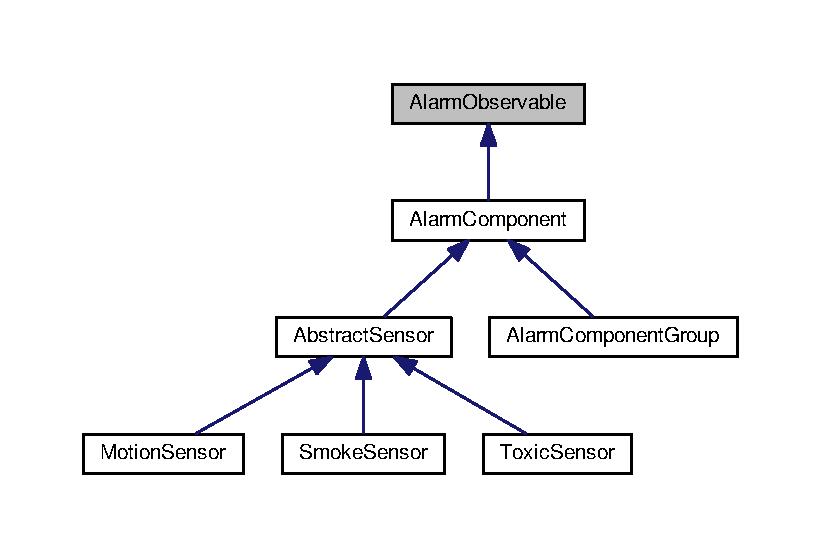
\includegraphics[width=350pt]{classAlarmObservable__inherit__graph}
\end{center}
\end{figure}
\subsection*{Public Types}
\begin{DoxyCompactItemize}
\item 
typedef std\+::shared\+\_\+ptr$<$ \hyperlink{classAlarmObserver}{Alarm\+Observer} $>$ {\bfseries S\+Ptr}\hypertarget{classAlarmObservable_a12ddadb3633a785fa4f79378b2b46878}{}\label{classAlarmObservable_a12ddadb3633a785fa4f79378b2b46878}

\end{DoxyCompactItemize}
\subsection*{Public Member Functions}
\begin{DoxyCompactItemize}
\item 
\hyperlink{classAlarmObservable_afd9c686eed16b00d73f8257d052021b4}{Alarm\+Observable} ()\hypertarget{classAlarmObservable_afd9c686eed16b00d73f8257d052021b4}{}\label{classAlarmObservable_afd9c686eed16b00d73f8257d052021b4}

\begin{DoxyCompactList}\small\item\em Class constructor. \end{DoxyCompactList}\item 
void \hyperlink{classAlarmObservable_aa8cf379c39c2c4a1e87925a6e79dfa11}{add\+Observer} (const S\+Ptr \&sptr)
\begin{DoxyCompactList}\small\item\em Add observer to the list of observers. \end{DoxyCompactList}\item 
void \hyperlink{classAlarmObservable_a76733a3271e053f105c428f3d878aa7e}{remove\+Observer} (const S\+Ptr \&sptr)
\begin{DoxyCompactList}\small\item\em Remove observer from the list of observers. \end{DoxyCompactList}\item 
virtual void \hyperlink{classAlarmObservable_afe90d2612d363050a620eb8b2ef2fa0a}{notify} (const std\+::string msg)
\begin{DoxyCompactList}\small\item\em Notify observers. \end{DoxyCompactList}\end{DoxyCompactItemize}


\subsection{Detailed Description}
Observable class of observer structure. 

Gives an opportunity to its successor to notify attached observer classes 

\subsection{Member Function Documentation}
\index{Alarm\+Observable@{Alarm\+Observable}!add\+Observer@{add\+Observer}}
\index{add\+Observer@{add\+Observer}!Alarm\+Observable@{Alarm\+Observable}}
\subsubsection[{\texorpdfstring{add\+Observer(const S\+Ptr \&sptr)}{addObserver(const SPtr &sptr)}}]{\setlength{\rightskip}{0pt plus 5cm}void Alarm\+Observable\+::add\+Observer (
\begin{DoxyParamCaption}
\item[{const S\+Ptr \&}]{sptr}
\end{DoxyParamCaption}
)}\hypertarget{classAlarmObservable_aa8cf379c39c2c4a1e87925a6e79dfa11}{}\label{classAlarmObservable_aa8cf379c39c2c4a1e87925a6e79dfa11}


Add observer to the list of observers. 


\begin{DoxyParams}{Parameters}
{\em sptr} & pointer to observer \\
\hline
\end{DoxyParams}
\index{Alarm\+Observable@{Alarm\+Observable}!notify@{notify}}
\index{notify@{notify}!Alarm\+Observable@{Alarm\+Observable}}
\subsubsection[{\texorpdfstring{notify(const std\+::string msg)}{notify(const std::string msg)}}]{\setlength{\rightskip}{0pt plus 5cm}void Alarm\+Observable\+::notify (
\begin{DoxyParamCaption}
\item[{const std\+::string}]{msg}
\end{DoxyParamCaption}
)\hspace{0.3cm}{\ttfamily [virtual]}}\hypertarget{classAlarmObservable_afe90d2612d363050a620eb8b2ef2fa0a}{}\label{classAlarmObservable_afe90d2612d363050a620eb8b2ef2fa0a}


Notify observers. 


\begin{DoxyParams}{Parameters}
{\em msg} & message to be sent \\
\hline
\end{DoxyParams}


Reimplemented in \hyperlink{classAlarmComponent_ae94d389ca9933e31e2bda486eb5b7c1f}{Alarm\+Component}.

\index{Alarm\+Observable@{Alarm\+Observable}!remove\+Observer@{remove\+Observer}}
\index{remove\+Observer@{remove\+Observer}!Alarm\+Observable@{Alarm\+Observable}}
\subsubsection[{\texorpdfstring{remove\+Observer(const S\+Ptr \&sptr)}{removeObserver(const SPtr &sptr)}}]{\setlength{\rightskip}{0pt plus 5cm}void Alarm\+Observable\+::remove\+Observer (
\begin{DoxyParamCaption}
\item[{const S\+Ptr \&}]{sptr}
\end{DoxyParamCaption}
)}\hypertarget{classAlarmObservable_a76733a3271e053f105c428f3d878aa7e}{}\label{classAlarmObservable_a76733a3271e053f105c428f3d878aa7e}


Remove observer from the list of observers. 


\begin{DoxyParams}{Parameters}
{\em sptr} & pointer to observer \\
\hline
\end{DoxyParams}


The documentation for this class was generated from the following files\+:\begin{DoxyCompactItemize}
\item 
alarm-\/observer/\hyperlink{alarmobservable_8h}{alarmobservable.\+h}\item 
alarm-\/observer/\hyperlink{alarmobservable_8cpp}{alarmobservable.\+cpp}\end{DoxyCompactItemize}

\hypertarget{classAlarmObserver}{}\section{Alarm\+Observer Class Reference}
\label{classAlarmObserver}\index{Alarm\+Observer@{Alarm\+Observer}}


Observer class of observer structure.  




{\ttfamily \#include $<$alarmobserver.\+h$>$}

\subsection*{Public Member Functions}
\begin{DoxyCompactItemize}
\item 
\hyperlink{classAlarmObserver_a8ea41b4a7ddebb267fd637c6e3f113f5}{Alarm\+Observer} (std\+::string name=\char`\"{}Uknown observer\char`\"{})
\begin{DoxyCompactList}\small\item\em Class constructor. \end{DoxyCompactList}\item 
void \hyperlink{classAlarmObserver_a203abff30c7ddb4a4139c56cbe11a2c2}{handle} (const std\+::string msg)
\begin{DoxyCompactList}\small\item\em Handle the event generated by observable. \end{DoxyCompactList}\end{DoxyCompactItemize}


\subsection{Detailed Description}
Observer class of observer structure. 

Gives an opportunity to its successor to be notified any observable object it is attached to 

\subsection{Constructor \& Destructor Documentation}
\index{Alarm\+Observer@{Alarm\+Observer}!Alarm\+Observer@{Alarm\+Observer}}
\index{Alarm\+Observer@{Alarm\+Observer}!Alarm\+Observer@{Alarm\+Observer}}
\subsubsection[{\texorpdfstring{Alarm\+Observer(std\+::string name=""Uknown observer"")}{AlarmObserver(std::string name="Uknown observer")}}]{\setlength{\rightskip}{0pt plus 5cm}Alarm\+Observer\+::\+Alarm\+Observer (
\begin{DoxyParamCaption}
\item[{std\+::string}]{name = {\ttfamily \char`\"{}Uknown~observer\char`\"{}}}
\end{DoxyParamCaption}
)}\hypertarget{classAlarmObserver_a8ea41b4a7ddebb267fd637c6e3f113f5}{}\label{classAlarmObserver_a8ea41b4a7ddebb267fd637c6e3f113f5}


Class constructor. 


\begin{DoxyParams}{Parameters}
{\em name} & name of the observer \\
\hline
\end{DoxyParams}


\subsection{Member Function Documentation}
\index{Alarm\+Observer@{Alarm\+Observer}!handle@{handle}}
\index{handle@{handle}!Alarm\+Observer@{Alarm\+Observer}}
\subsubsection[{\texorpdfstring{handle(const std\+::string msg)}{handle(const std::string msg)}}]{\setlength{\rightskip}{0pt plus 5cm}void Alarm\+Observer\+::handle (
\begin{DoxyParamCaption}
\item[{const std\+::string}]{msg}
\end{DoxyParamCaption}
)}\hypertarget{classAlarmObserver_a203abff30c7ddb4a4139c56cbe11a2c2}{}\label{classAlarmObserver_a203abff30c7ddb4a4139c56cbe11a2c2}


Handle the event generated by observable. 


\begin{DoxyParams}{Parameters}
{\em msg} & message that was sent from an observable \\
\hline
\end{DoxyParams}


The documentation for this class was generated from the following files\+:\begin{DoxyCompactItemize}
\item 
alarm-\/observer/\hyperlink{alarmobserver_8h}{alarmobserver.\+h}\item 
alarm-\/observer/\hyperlink{alarmobserver_8cpp}{alarmobserver.\+cpp}\end{DoxyCompactItemize}

\hypertarget{classAlarmSignal}{}\section{Alarm\+Signal Class Reference}
\label{classAlarmSignal}\index{Alarm\+Signal@{Alarm\+Signal}}


Call police strategy class.  




{\ttfamily \#include $<$alarmsignal.\+h$>$}



Inheritance diagram for Alarm\+Signal\+:\nopagebreak
\begin{figure}[H]
\begin{center}
\leavevmode
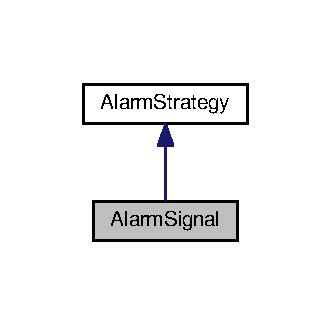
\includegraphics[width=159pt]{classAlarmSignal__inherit__graph}
\end{center}
\end{figure}


Collaboration diagram for Alarm\+Signal\+:\nopagebreak
\begin{figure}[H]
\begin{center}
\leavevmode
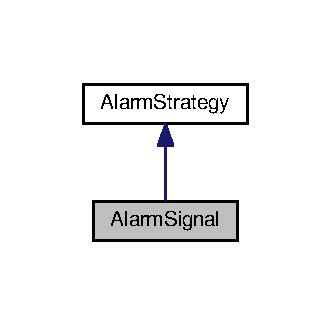
\includegraphics[width=159pt]{classAlarmSignal__coll__graph}
\end{center}
\end{figure}
\subsection*{Additional Inherited Members}


\subsection{Detailed Description}
Call police strategy class. 

Dummy implementation of call police strategy. Intended for testing purposes. 

The documentation for this class was generated from the following files\+:\begin{DoxyCompactItemize}
\item 
alarm-\/strategy/\hyperlink{alarmsignal_8h}{alarmsignal.\+h}\item 
alarm-\/strategy/\hyperlink{alarmsignal_8cpp}{alarmsignal.\+cpp}\end{DoxyCompactItemize}

\hypertarget{classAlarmStrategy}{}\section{Alarm\+Strategy Class Reference}
\label{classAlarmStrategy}\index{Alarm\+Strategy@{Alarm\+Strategy}}


Strategy class implementation of strategy pattern.  




{\ttfamily \#include $<$alarmstrategy.\+h$>$}



Inheritance diagram for Alarm\+Strategy\+:\nopagebreak
\begin{figure}[H]
\begin{center}
\leavevmode
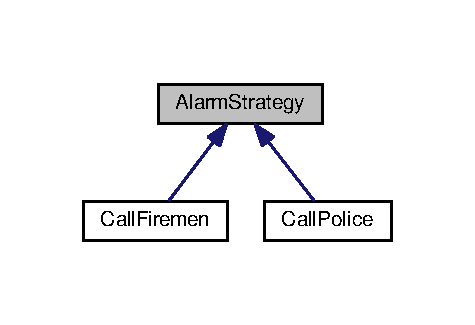
\includegraphics[width=254pt]{classAlarmStrategy__inherit__graph}
\end{center}
\end{figure}
\subsection*{Public Member Functions}
\begin{DoxyCompactItemize}
\item 
\hyperlink{classAlarmStrategy_afe181296dbc2f3a87ccc50f9d92349fd}{Alarm\+Strategy} (std\+::string name=\char`\"{}Unknown strategy\char`\"{})
\begin{DoxyCompactList}\small\item\em Class constructor. \end{DoxyCompactList}\item 
virtual void \hyperlink{classAlarmStrategy_a6aedaab2ebe535c76af8d3e07dcf7f1e}{activate} ()\hypertarget{classAlarmStrategy_a6aedaab2ebe535c76af8d3e07dcf7f1e}{}\label{classAlarmStrategy_a6aedaab2ebe535c76af8d3e07dcf7f1e}

\begin{DoxyCompactList}\small\item\em Trigger the strategy execution. \end{DoxyCompactList}\item 
virtual void \hyperlink{classAlarmStrategy_ad04a9ef585215c424adea86447d7c994}{deactivate} ()\hypertarget{classAlarmStrategy_ad04a9ef585215c424adea86447d7c994}{}\label{classAlarmStrategy_ad04a9ef585215c424adea86447d7c994}

\begin{DoxyCompactList}\small\item\em Deactivate the strategy execution. \end{DoxyCompactList}\end{DoxyCompactItemize}


\subsection{Detailed Description}
Strategy class implementation of strategy pattern. 

\subsection{Constructor \& Destructor Documentation}
\index{Alarm\+Strategy@{Alarm\+Strategy}!Alarm\+Strategy@{Alarm\+Strategy}}
\index{Alarm\+Strategy@{Alarm\+Strategy}!Alarm\+Strategy@{Alarm\+Strategy}}
\subsubsection[{\texorpdfstring{Alarm\+Strategy(std\+::string name=""Unknown strategy"")}{AlarmStrategy(std::string name="Unknown strategy")}}]{\setlength{\rightskip}{0pt plus 5cm}Alarm\+Strategy\+::\+Alarm\+Strategy (
\begin{DoxyParamCaption}
\item[{std\+::string}]{name = {\ttfamily \char`\"{}Unknown~strategy\char`\"{}}}
\end{DoxyParamCaption}
)\hspace{0.3cm}{\ttfamily [explicit]}}\hypertarget{classAlarmStrategy_afe181296dbc2f3a87ccc50f9d92349fd}{}\label{classAlarmStrategy_afe181296dbc2f3a87ccc50f9d92349fd}


Class constructor. 


\begin{DoxyParams}{Parameters}
{\em name} & name of the strategy \\
\hline
\end{DoxyParams}


The documentation for this class was generated from the following files\+:\begin{DoxyCompactItemize}
\item 
alarm-\/strategy/\hyperlink{alarmstrategy_8h}{alarmstrategy.\+h}\item 
alarm-\/strategy/\hyperlink{alarmstrategy_8cpp}{alarmstrategy.\+cpp}\end{DoxyCompactItemize}

\hypertarget{classAlarmStrategyOwner}{}\section{Alarm\+Strategy\+Owner Class Reference}
\label{classAlarmStrategyOwner}\index{Alarm\+Strategy\+Owner@{Alarm\+Strategy\+Owner}}


Context class implementation of strategy pattern.  




{\ttfamily \#include $<$alarmstrategyowner.\+h$>$}



Inheritance diagram for Alarm\+Strategy\+Owner\+:\nopagebreak
\begin{figure}[H]
\begin{center}
\leavevmode
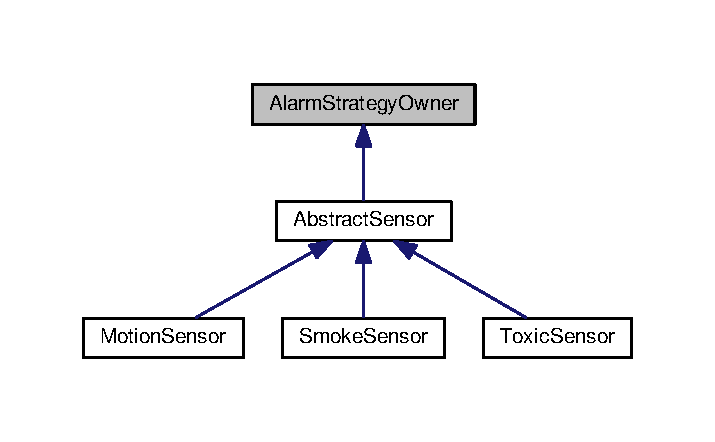
\includegraphics[width=350pt]{classAlarmStrategyOwner__inherit__graph}
\end{center}
\end{figure}
\subsection*{Public Types}
\begin{DoxyCompactItemize}
\item 
typedef std\+::shared\+\_\+ptr$<$ \hyperlink{classAlarmStrategy}{Alarm\+Strategy} $>$ {\bfseries S\+Ptr}\hypertarget{classAlarmStrategyOwner_aeebd31011e2a6d14a4492315ad15c5ee}{}\label{classAlarmStrategyOwner_aeebd31011e2a6d14a4492315ad15c5ee}

\end{DoxyCompactItemize}
\subsection*{Public Member Functions}
\begin{DoxyCompactItemize}
\item 
void \hyperlink{classAlarmStrategyOwner_a2e150fb66eda048ece19da4ebf3605cf}{activate\+Strategies} ()\hypertarget{classAlarmStrategyOwner_a2e150fb66eda048ece19da4ebf3605cf}{}\label{classAlarmStrategyOwner_a2e150fb66eda048ece19da4ebf3605cf}

\begin{DoxyCompactList}\small\item\em Activate all strategies held by the instance. \end{DoxyCompactList}\item 
void \hyperlink{classAlarmStrategyOwner_a24165674f81b7414ea7f49addf7afc0a}{deactivate\+Strategies} ()\hypertarget{classAlarmStrategyOwner_a24165674f81b7414ea7f49addf7afc0a}{}\label{classAlarmStrategyOwner_a24165674f81b7414ea7f49addf7afc0a}

\begin{DoxyCompactList}\small\item\em Deactivate all strategies held by the instance. \end{DoxyCompactList}\item 
void \hyperlink{classAlarmStrategyOwner_a38dde4dca444585387df6db6bf352349}{add\+Strategy} (const S\+Ptr \&strategy)
\begin{DoxyCompactList}\small\item\em Add strategy to the context. \end{DoxyCompactList}\item 
void \hyperlink{classAlarmStrategyOwner_a50ca40d662757f37fdb17194fdbb165a}{remove\+Strategy} (const S\+Ptr \&strategy)
\begin{DoxyCompactList}\small\item\em Remove strategy from the context. \end{DoxyCompactList}\end{DoxyCompactItemize}


\subsection{Detailed Description}
Context class implementation of strategy pattern. 

\subsection{Member Function Documentation}
\index{Alarm\+Strategy\+Owner@{Alarm\+Strategy\+Owner}!add\+Strategy@{add\+Strategy}}
\index{add\+Strategy@{add\+Strategy}!Alarm\+Strategy\+Owner@{Alarm\+Strategy\+Owner}}
\subsubsection[{\texorpdfstring{add\+Strategy(const S\+Ptr \&strategy)}{addStrategy(const SPtr &strategy)}}]{\setlength{\rightskip}{0pt plus 5cm}void Alarm\+Strategy\+Owner\+::add\+Strategy (
\begin{DoxyParamCaption}
\item[{const S\+Ptr \&}]{strategy}
\end{DoxyParamCaption}
)}\hypertarget{classAlarmStrategyOwner_a38dde4dca444585387df6db6bf352349}{}\label{classAlarmStrategyOwner_a38dde4dca444585387df6db6bf352349}


Add strategy to the context. 


\begin{DoxyParams}{Parameters}
{\em strategy} & strategy to be added \\
\hline
\end{DoxyParams}
\index{Alarm\+Strategy\+Owner@{Alarm\+Strategy\+Owner}!remove\+Strategy@{remove\+Strategy}}
\index{remove\+Strategy@{remove\+Strategy}!Alarm\+Strategy\+Owner@{Alarm\+Strategy\+Owner}}
\subsubsection[{\texorpdfstring{remove\+Strategy(const S\+Ptr \&strategy)}{removeStrategy(const SPtr &strategy)}}]{\setlength{\rightskip}{0pt plus 5cm}void Alarm\+Strategy\+Owner\+::remove\+Strategy (
\begin{DoxyParamCaption}
\item[{const S\+Ptr \&}]{strategy}
\end{DoxyParamCaption}
)}\hypertarget{classAlarmStrategyOwner_a50ca40d662757f37fdb17194fdbb165a}{}\label{classAlarmStrategyOwner_a50ca40d662757f37fdb17194fdbb165a}


Remove strategy from the context. 


\begin{DoxyParams}{Parameters}
{\em strategy} & to be removed \\
\hline
\end{DoxyParams}


The documentation for this class was generated from the following files\+:\begin{DoxyCompactItemize}
\item 
alarm-\/strategy/\hyperlink{alarmstrategyowner_8h}{alarmstrategyowner.\+h}\item 
alarm-\/strategy/\hyperlink{alarmstrategyowner_8cpp}{alarmstrategyowner.\+cpp}\end{DoxyCompactItemize}

\hypertarget{classcompareByType}{}\section{compare\+By\+Type Class Reference}
\label{classcompareByType}\index{compare\+By\+Type@{compare\+By\+Type}}


Sorting by type functor for Alarm\+Sensors.  




{\ttfamily \#include $<$abstractsensor.\+h$>$}

\subsection*{Public Member Functions}
\begin{DoxyCompactItemize}
\item 
bool {\bfseries operator()} (const Alarm\+Component\+::\+S\+Ptr \&sptr1, const Alarm\+Component\+::\+S\+Ptr \&sptr2)\hypertarget{classcompareByType_a8894c7df4c6735d26043a5720b0a5a26}{}\label{classcompareByType_a8894c7df4c6735d26043a5720b0a5a26}

\end{DoxyCompactItemize}


\subsection{Detailed Description}
Sorting by type functor for Alarm\+Sensors. 

The documentation for this class was generated from the following file\+:\begin{DoxyCompactItemize}
\item 
alarm-\/sensor/\hyperlink{abstractsensor_8h}{abstractsensor.\+h}\end{DoxyCompactItemize}

\hypertarget{classcompareByVendor}{}\section{compare\+By\+Vendor Class Reference}
\label{classcompareByVendor}\index{compare\+By\+Vendor@{compare\+By\+Vendor}}


Sorting by vendor functor for Alarm\+Sensors.  




{\ttfamily \#include $<$abstractsensor.\+h$>$}

\subsection*{Public Member Functions}
\begin{DoxyCompactItemize}
\item 
bool {\bfseries operator()} (const Alarm\+Component\+::\+S\+Ptr \&sptr1, const Alarm\+Component\+::\+S\+Ptr \&sptr2)\hypertarget{classcompareByVendor_a10b4288c8c40f52bf6360d3c137ad883}{}\label{classcompareByVendor_a10b4288c8c40f52bf6360d3c137ad883}

\end{DoxyCompactItemize}


\subsection{Detailed Description}
Sorting by vendor functor for Alarm\+Sensors. 

The documentation for this class was generated from the following file\+:\begin{DoxyCompactItemize}
\item 
alarm-\/sensor/\hyperlink{abstractsensor_8h}{abstractsensor.\+h}\end{DoxyCompactItemize}

\hypertarget{classcompareByVendorByType}{}\section{compare\+By\+Vendor\+By\+Type Class Reference}
\label{classcompareByVendorByType}\index{compare\+By\+Vendor\+By\+Type@{compare\+By\+Vendor\+By\+Type}}


Sorting by vendor by type functor for Alarm\+Sensors.  




{\ttfamily \#include $<$abstractsensor.\+h$>$}

\subsection*{Public Member Functions}
\begin{DoxyCompactItemize}
\item 
bool {\bfseries operator()} (const Alarm\+Component\+::\+S\+Ptr \&sptr1, const Alarm\+Component\+::\+S\+Ptr \&sptr2)\hypertarget{classcompareByVendorByType_a89e0ddac8ee1707d6efb2f44bb654465}{}\label{classcompareByVendorByType_a89e0ddac8ee1707d6efb2f44bb654465}

\end{DoxyCompactItemize}


\subsection{Detailed Description}
Sorting by vendor by type functor for Alarm\+Sensors. 

The documentation for this class was generated from the following file\+:\begin{DoxyCompactItemize}
\item 
alarm-\/sensor/\hyperlink{abstractsensor_8h}{abstractsensor.\+h}\end{DoxyCompactItemize}

\hypertarget{classMotionSensor}{}\section{Motion\+Sensor Class Reference}
\label{classMotionSensor}\index{Motion\+Sensor@{Motion\+Sensor}}


Motion sensor class.  




{\ttfamily \#include $<$motionsensor.\+h$>$}



Inheritance diagram for Motion\+Sensor\+:
\nopagebreak
\begin{figure}[H]
\begin{center}
\leavevmode
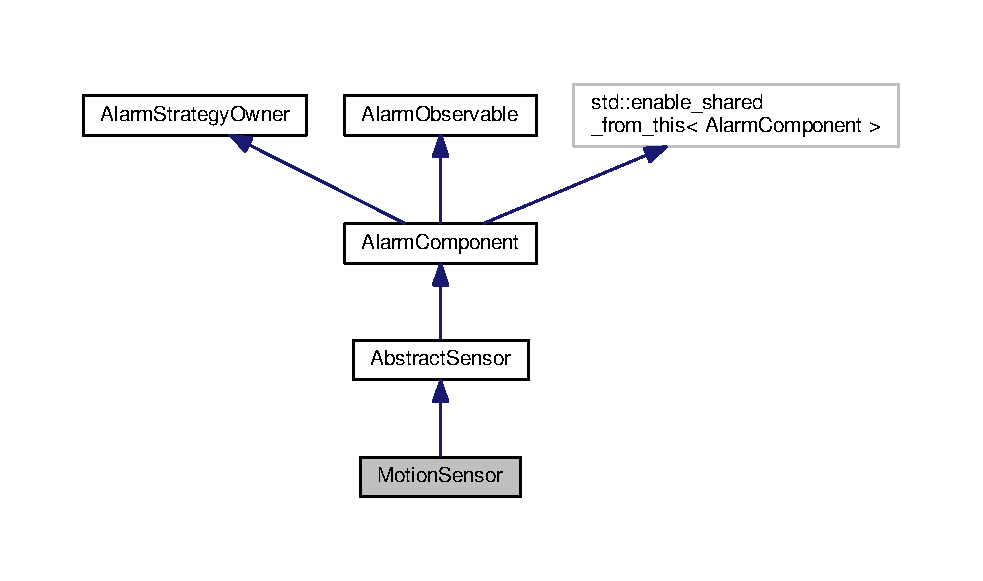
\includegraphics[width=330pt]{classMotionSensor__inherit__graph}
\end{center}
\end{figure}


Collaboration diagram for Motion\+Sensor\+:
\nopagebreak
\begin{figure}[H]
\begin{center}
\leavevmode
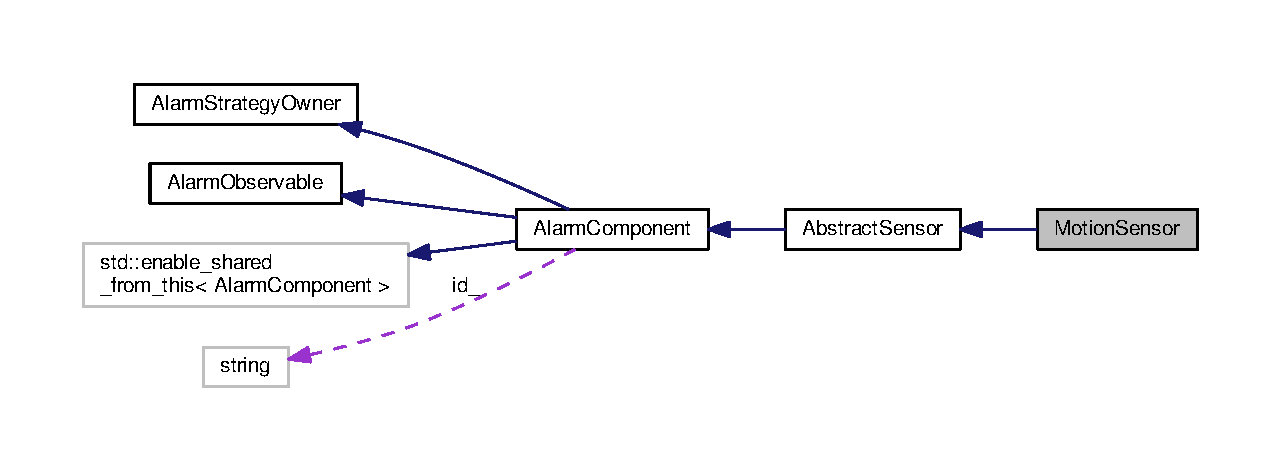
\includegraphics[width=350pt]{classMotionSensor__coll__graph}
\end{center}
\end{figure}
\subsection*{Public Member Functions}
\begin{DoxyCompactItemize}
\item 
\hyperlink{classMotionSensor_a411baafe617c6e11c10aaa0e1ec6a9f4}{Motion\+Sensor} (int min\+Distance=0, int max\+Distance=20, std\+::string id=\char`\"{}Unkown id\char`\"{}, std\+::string vendor=\char`\"{}Unkown vendor\char`\"{})
\begin{DoxyCompactList}\small\item\em Class constructor. \end{DoxyCompactList}\item 
virtual void \hyperlink{classMotionSensor_a8e71f20dc63f45669377e6efc4d7c6df}{update} () override
\begin{DoxyCompactList}\small\item\em Update of the current value. \end{DoxyCompactList}\item 
virtual const std\+::string \hyperlink{classMotionSensor_a9b0a0233e5ccfb714cf5d10acfc0e188}{get\+Info} () const override\hypertarget{classMotionSensor_a9b0a0233e5ccfb714cf5d10acfc0e188}{}\label{classMotionSensor_a9b0a0233e5ccfb714cf5d10acfc0e188}

\begin{DoxyCompactList}\small\item\em String stream containing info about the sensor. \end{DoxyCompactList}\item 
int \hyperlink{classMotionSensor_aa19bf311e57fc21276d2eb74190cb709}{get\+Min\+Distance} () const \hypertarget{classMotionSensor_aa19bf311e57fc21276d2eb74190cb709}{}\label{classMotionSensor_aa19bf311e57fc21276d2eb74190cb709}

\begin{DoxyCompactList}\small\item\em Returns mininal sensitive distance. \end{DoxyCompactList}\item 
int \hyperlink{classMotionSensor_af095104075a3e5cb7c6c6466c8813f26}{get\+Max\+Distance} () const \hypertarget{classMotionSensor_af095104075a3e5cb7c6c6466c8813f26}{}\label{classMotionSensor_af095104075a3e5cb7c6c6466c8813f26}

\begin{DoxyCompactList}\small\item\em Returns maximal sensitive distance. \end{DoxyCompactList}\end{DoxyCompactItemize}
\subsection*{Additional Inherited Members}


\subsection{Detailed Description}
Motion sensor class. 

Dummy implementation of motion sensor component. Intended for testing purposes. 

\subsection{Constructor \& Destructor Documentation}
\index{Motion\+Sensor@{Motion\+Sensor}!Motion\+Sensor@{Motion\+Sensor}}
\index{Motion\+Sensor@{Motion\+Sensor}!Motion\+Sensor@{Motion\+Sensor}}
\subsubsection[{\texorpdfstring{Motion\+Sensor(int min\+Distance=0, int max\+Distance=20, std\+::string id=""Unkown id"", std\+::string vendor=""Unkown vendor"")}{MotionSensor(int minDistance=0, int maxDistance=20, std::string id="Unkown id", std::string vendor="Unkown vendor")}}]{\setlength{\rightskip}{0pt plus 5cm}Motion\+Sensor\+::\+Motion\+Sensor (
\begin{DoxyParamCaption}
\item[{int}]{min\+Distance = {\ttfamily 0}, }
\item[{int}]{max\+Distance = {\ttfamily 20}, }
\item[{std\+::string}]{id = {\ttfamily \char`\"{}Unkown~id\char`\"{}}, }
\item[{std\+::string}]{vendor = {\ttfamily \char`\"{}Unkown~vendor\char`\"{}}}
\end{DoxyParamCaption}
)}\hypertarget{classMotionSensor_a411baafe617c6e11c10aaa0e1ec6a9f4}{}\label{classMotionSensor_a411baafe617c6e11c10aaa0e1ec6a9f4}


Class constructor. 


\begin{DoxyParams}{Parameters}
{\em min\+Distance} & minimal distance of activation \\
\hline
{\em max\+Distance} & maximal distance of activation \\
\hline
{\em id} & identificator of the sensor \\
\hline
{\em vendor} & vendor name \\
\hline
\end{DoxyParams}


\subsection{Member Function Documentation}
\index{Motion\+Sensor@{Motion\+Sensor}!update@{update}}
\index{update@{update}!Motion\+Sensor@{Motion\+Sensor}}
\subsubsection[{\texorpdfstring{update() override}{update() override}}]{\setlength{\rightskip}{0pt plus 5cm}void Motion\+Sensor\+::update (
\begin{DoxyParamCaption}
{}
\end{DoxyParamCaption}
)\hspace{0.3cm}{\ttfamily [override]}, {\ttfamily [virtual]}}\hypertarget{classMotionSensor_a8e71f20dc63f45669377e6efc4d7c6df}{}\label{classMotionSensor_a8e71f20dc63f45669377e6efc4d7c6df}


Update of the current value. 

Randomly defines current value of the signal and triggers the activation if the value is within the active range 

Implements \hyperlink{classAbstractSensor_a8d0a1908c6aaf67fc7d781e54b49293b}{Abstract\+Sensor}.



The documentation for this class was generated from the following files\+:\begin{DoxyCompactItemize}
\item 
alarm-\/sensor/\hyperlink{motionsensor_8h}{motionsensor.\+h}\item 
alarm-\/sensor/motionsensor.\+cpp\end{DoxyCompactItemize}

\hypertarget{classSmokeSensor}{}\section{Smoke\+Sensor Class Reference}
\label{classSmokeSensor}\index{Smoke\+Sensor@{Smoke\+Sensor}}


Smoke sensor class.  




{\ttfamily \#include $<$smokesensor.\+h$>$}



Inheritance diagram for Smoke\+Sensor\+:
\nopagebreak
\begin{figure}[H]
\begin{center}
\leavevmode
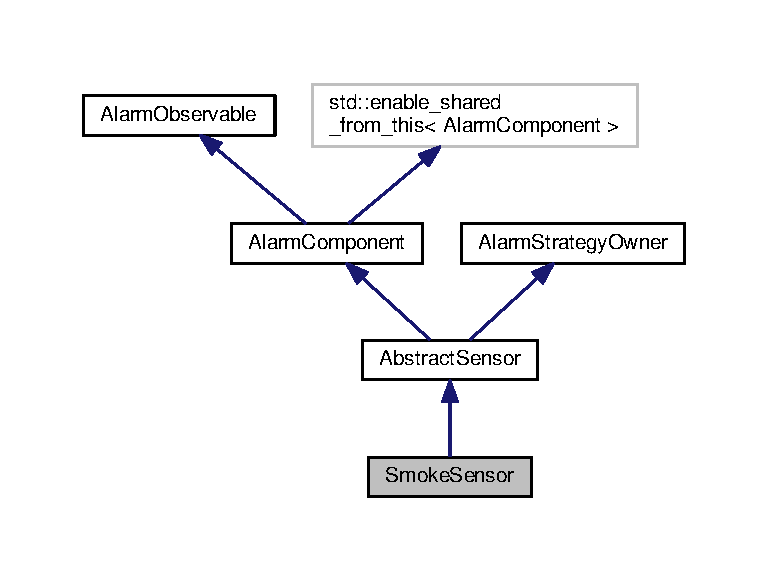
\includegraphics[width=330pt]{classSmokeSensor__inherit__graph}
\end{center}
\end{figure}


Collaboration diagram for Smoke\+Sensor\+:
\nopagebreak
\begin{figure}[H]
\begin{center}
\leavevmode
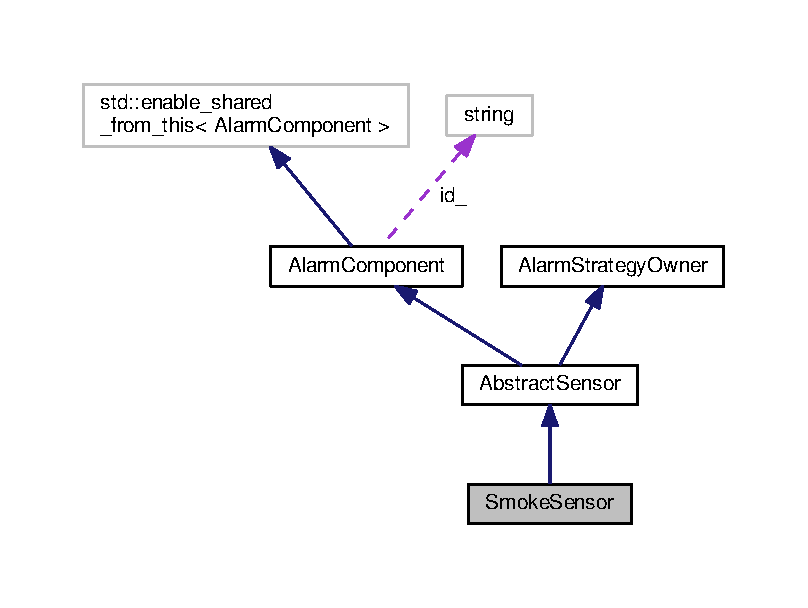
\includegraphics[width=350pt]{classSmokeSensor__coll__graph}
\end{center}
\end{figure}
\subsection*{Public Member Functions}
\begin{DoxyCompactItemize}
\item 
\hyperlink{classSmokeSensor_a0a8061f510440bd20f6ca7238b23516c}{Smoke\+Sensor} (int threshold=20, std\+::string id=\char`\"{}Unkown id\char`\"{}, std\+::string vendor=\char`\"{}Unkown vendor\char`\"{})
\begin{DoxyCompactList}\small\item\em Class constructor. \end{DoxyCompactList}\item 
virtual void \hyperlink{classSmokeSensor_a31bc900b0d1c5c893f8555fdcbe4266b}{update} () override
\begin{DoxyCompactList}\small\item\em Update of the current value. \end{DoxyCompactList}\item 
virtual const std\+::string \hyperlink{classSmokeSensor_a2cc7e7b2da913abb8aefcd92d50ef046}{get\+Info} () const override\hypertarget{classSmokeSensor_a2cc7e7b2da913abb8aefcd92d50ef046}{}\label{classSmokeSensor_a2cc7e7b2da913abb8aefcd92d50ef046}

\begin{DoxyCompactList}\small\item\em String stream containing info about the sensor. \end{DoxyCompactList}\item 
int \hyperlink{classSmokeSensor_add325306c6a33436bc9053721cbdb88b}{get\+Threshold} () const 
\begin{DoxyCompactList}\small\item\em Threshold access function. \end{DoxyCompactList}\end{DoxyCompactItemize}
\subsection*{Additional Inherited Members}


\subsection{Detailed Description}
Smoke sensor class. 

Dummy implementation of smoke sensor component. Intended for testing purposes. 

\subsection{Constructor \& Destructor Documentation}
\index{Smoke\+Sensor@{Smoke\+Sensor}!Smoke\+Sensor@{Smoke\+Sensor}}
\index{Smoke\+Sensor@{Smoke\+Sensor}!Smoke\+Sensor@{Smoke\+Sensor}}
\subsubsection[{\texorpdfstring{Smoke\+Sensor(int threshold=20, std\+::string id=""Unkown id"", std\+::string vendor=""Unkown vendor"")}{SmokeSensor(int threshold=20, std::string id="Unkown id", std::string vendor="Unkown vendor")}}]{\setlength{\rightskip}{0pt plus 5cm}Smoke\+Sensor\+::\+Smoke\+Sensor (
\begin{DoxyParamCaption}
\item[{int}]{threshold = {\ttfamily 20}, }
\item[{std\+::string}]{id = {\ttfamily \char`\"{}Unkown~id\char`\"{}}, }
\item[{std\+::string}]{vendor = {\ttfamily \char`\"{}Unkown~vendor\char`\"{}}}
\end{DoxyParamCaption}
)}\hypertarget{classSmokeSensor_a0a8061f510440bd20f6ca7238b23516c}{}\label{classSmokeSensor_a0a8061f510440bd20f6ca7238b23516c}


Class constructor. 


\begin{DoxyParams}{Parameters}
{\em threshold} & minimal value for activation \\
\hline
{\em id} & identificator of the sensor \\
\hline
{\em vendor} & vendor name \\
\hline
\end{DoxyParams}


\subsection{Member Function Documentation}
\index{Smoke\+Sensor@{Smoke\+Sensor}!get\+Threshold@{get\+Threshold}}
\index{get\+Threshold@{get\+Threshold}!Smoke\+Sensor@{Smoke\+Sensor}}
\subsubsection[{\texorpdfstring{get\+Threshold() const }{getThreshold() const }}]{\setlength{\rightskip}{0pt plus 5cm}int Smoke\+Sensor\+::get\+Threshold (
\begin{DoxyParamCaption}
{}
\end{DoxyParamCaption}
) const\hspace{0.3cm}{\ttfamily [inline]}}\hypertarget{classSmokeSensor_add325306c6a33436bc9053721cbdb88b}{}\label{classSmokeSensor_add325306c6a33436bc9053721cbdb88b}


Threshold access function. 

\begin{DoxyReturn}{Returns}
current threshold value 
\end{DoxyReturn}
\index{Smoke\+Sensor@{Smoke\+Sensor}!update@{update}}
\index{update@{update}!Smoke\+Sensor@{Smoke\+Sensor}}
\subsubsection[{\texorpdfstring{update() override}{update() override}}]{\setlength{\rightskip}{0pt plus 5cm}void Smoke\+Sensor\+::update (
\begin{DoxyParamCaption}
{}
\end{DoxyParamCaption}
)\hspace{0.3cm}{\ttfamily [override]}, {\ttfamily [virtual]}}\hypertarget{classSmokeSensor_a31bc900b0d1c5c893f8555fdcbe4266b}{}\label{classSmokeSensor_a31bc900b0d1c5c893f8555fdcbe4266b}


Update of the current value. 

Randomly defines current value of the signal and triggers the activation if the value higher than the threshold 

Implements \hyperlink{classAbstractSensor_a8d0a1908c6aaf67fc7d781e54b49293b}{Abstract\+Sensor}.



The documentation for this class was generated from the following files\+:\begin{DoxyCompactItemize}
\item 
alarm-\/sensor/\hyperlink{smokesensor_8h}{smokesensor.\+h}\item 
alarm-\/sensor/smokesensor.\+cpp\end{DoxyCompactItemize}

\hypertarget{classToxicSensor}{}\section{Toxic\+Sensor Class Reference}
\label{classToxicSensor}\index{Toxic\+Sensor@{Toxic\+Sensor}}


Toxic sensor class.  




{\ttfamily \#include $<$toxicsensor.\+h$>$}



Inheritance diagram for Toxic\+Sensor\+:\nopagebreak
\begin{figure}[H]
\begin{center}
\leavevmode
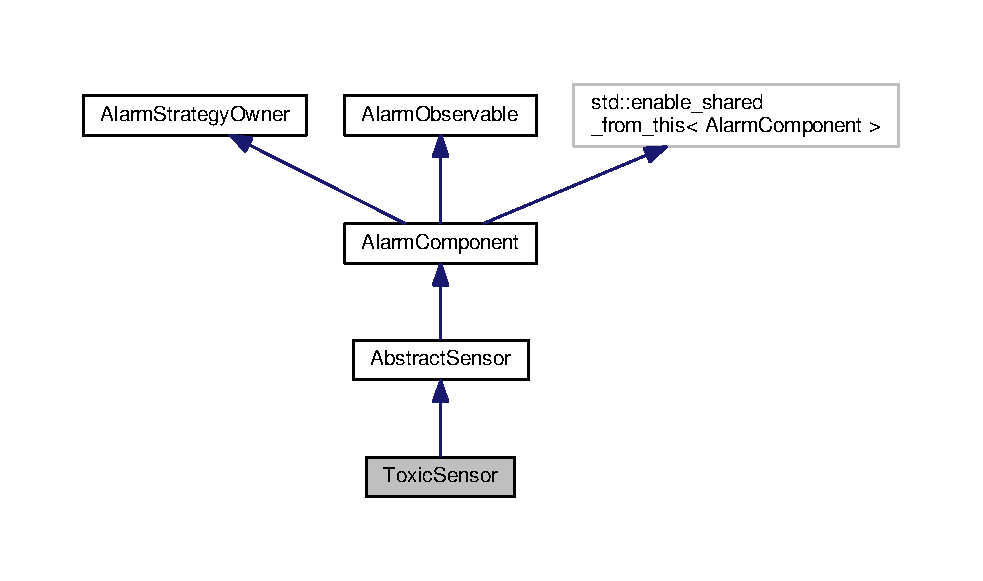
\includegraphics[width=298pt]{classToxicSensor__inherit__graph}
\end{center}
\end{figure}


Collaboration diagram for Toxic\+Sensor\+:\nopagebreak
\begin{figure}[H]
\begin{center}
\leavevmode
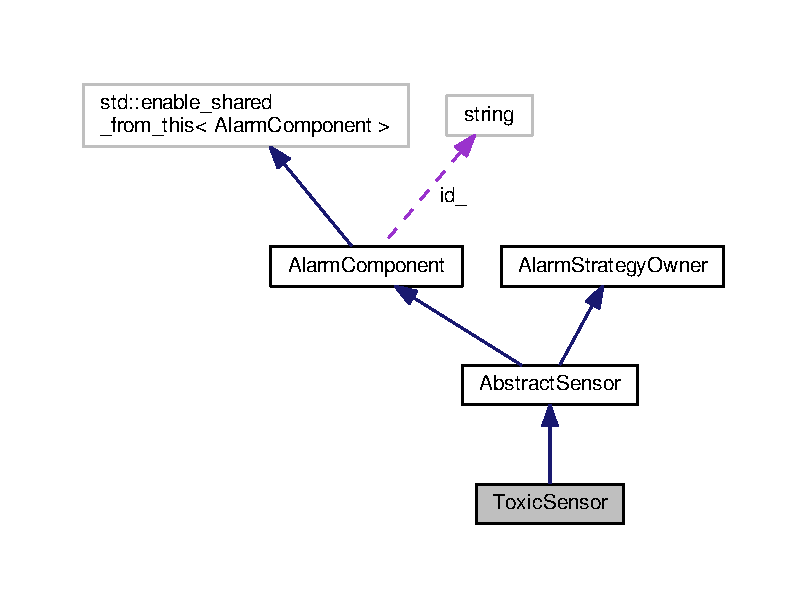
\includegraphics[width=298pt]{classToxicSensor__coll__graph}
\end{center}
\end{figure}
\subsection*{Public Types}
\begin{DoxyCompactItemize}
\item 
enum \hyperlink{classToxicSensor_a140f14965ad9a7e71fc8a5a2ed2c919b}{Gas\+Type} \{ {\bfseries Chlorine}, 
{\bfseries Bromine}
 \}\begin{DoxyCompactList}\small\item\em The Gas\+Type enum. \end{DoxyCompactList}
\end{DoxyCompactItemize}
\subsection*{Public Member Functions}
\begin{DoxyCompactItemize}
\item 
\hyperlink{classToxicSensor_a3d1f5f90e0561127e8ee3e5ee79c6473}{Toxic\+Sensor} (\hyperlink{classToxicSensor_a140f14965ad9a7e71fc8a5a2ed2c919b}{Gas\+Type} gas=Chlorine, int threshold=20, std\+::string id=\char`\"{}Unkown id\char`\"{}, std\+::string vendor=\char`\"{}Unkown vendor\char`\"{})
\begin{DoxyCompactList}\small\item\em Class constructor. \end{DoxyCompactList}\item 
virtual void \hyperlink{classToxicSensor_ae4c58761cf2ef02e1d782f7f13cc56ff}{update} () override
\begin{DoxyCompactList}\small\item\em Update of the current value. \end{DoxyCompactList}\end{DoxyCompactItemize}
\subsection*{Additional Inherited Members}


\subsection{Detailed Description}
Toxic sensor class. 

Dummy implementation of toxic sensor component. Intended for testing purposes. 

\subsection{Member Enumeration Documentation}
\index{Toxic\+Sensor@{Toxic\+Sensor}!Gas\+Type@{Gas\+Type}}
\index{Gas\+Type@{Gas\+Type}!Toxic\+Sensor@{Toxic\+Sensor}}
\subsubsection[{\texorpdfstring{Gas\+Type}{GasType}}]{\setlength{\rightskip}{0pt plus 5cm}enum {\bf Toxic\+Sensor\+::\+Gas\+Type}}\hypertarget{classToxicSensor_a140f14965ad9a7e71fc8a5a2ed2c919b}{}\label{classToxicSensor_a140f14965ad9a7e71fc8a5a2ed2c919b}


The Gas\+Type enum. 

Specifies types of Gas to which toxic sensor can be sensitive 

\subsection{Constructor \& Destructor Documentation}
\index{Toxic\+Sensor@{Toxic\+Sensor}!Toxic\+Sensor@{Toxic\+Sensor}}
\index{Toxic\+Sensor@{Toxic\+Sensor}!Toxic\+Sensor@{Toxic\+Sensor}}
\subsubsection[{\texorpdfstring{Toxic\+Sensor(\+Gas\+Type gas=\+Chlorine, int threshold=20, std\+::string id=""Unkown id"", std\+::string vendor=""Unkown vendor"")}{ToxicSensor(GasType gas=Chlorine, int threshold=20, std::string id="Unkown id", std::string vendor="Unkown vendor")}}]{\setlength{\rightskip}{0pt plus 5cm}Toxic\+Sensor\+::\+Toxic\+Sensor (
\begin{DoxyParamCaption}
\item[{{\bf Gas\+Type}}]{gas = {\ttfamily Chlorine}, }
\item[{int}]{threshold = {\ttfamily 20}, }
\item[{std\+::string}]{id = {\ttfamily \char`\"{}Unkown~id\char`\"{}}, }
\item[{std\+::string}]{vendor = {\ttfamily \char`\"{}Unkown~vendor\char`\"{}}}
\end{DoxyParamCaption}
)}\hypertarget{classToxicSensor_a3d1f5f90e0561127e8ee3e5ee79c6473}{}\label{classToxicSensor_a3d1f5f90e0561127e8ee3e5ee79c6473}


Class constructor. 


\begin{DoxyParams}{Parameters}
{\em gas} & type of gas being detected by the sensor \\
\hline
{\em threshold} & minimal value for activation \\
\hline
{\em id} & identificator of the sensor \\
\hline
{\em vendor} & vendor name \\
\hline
\end{DoxyParams}


\subsection{Member Function Documentation}
\index{Toxic\+Sensor@{Toxic\+Sensor}!update@{update}}
\index{update@{update}!Toxic\+Sensor@{Toxic\+Sensor}}
\subsubsection[{\texorpdfstring{update() override}{update() override}}]{\setlength{\rightskip}{0pt plus 5cm}void Toxic\+Sensor\+::update (
\begin{DoxyParamCaption}
{}
\end{DoxyParamCaption}
)\hspace{0.3cm}{\ttfamily [override]}, {\ttfamily [virtual]}}\hypertarget{classToxicSensor_ae4c58761cf2ef02e1d782f7f13cc56ff}{}\label{classToxicSensor_ae4c58761cf2ef02e1d782f7f13cc56ff}


Update of the current value. 

Randomly defines current value of the signal and triggers the activation if the value higher than the threshold 

Implements \hyperlink{classAbstractSensor_a8d0a1908c6aaf67fc7d781e54b49293b}{Abstract\+Sensor}.



The documentation for this class was generated from the following files\+:\begin{DoxyCompactItemize}
\item 
\hyperlink{toxicsensor_8h}{toxicsensor.\+h}\item 
toxicsensor.\+cpp\end{DoxyCompactItemize}

\hypertarget{classWaterDispenser}{}\section{Water\+Dispenser Class Reference}
\label{classWaterDispenser}\index{Water\+Dispenser@{Water\+Dispenser}}


Call firemen strategy class.  




{\ttfamily \#include $<$waterdispenser.\+h$>$}



Inheritance diagram for Water\+Dispenser\+:\nopagebreak
\begin{figure}[H]
\begin{center}
\leavevmode
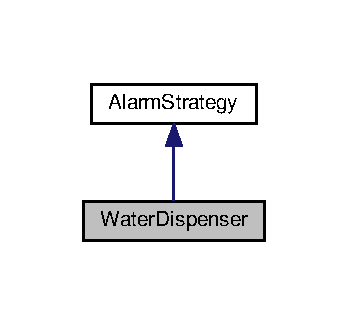
\includegraphics[width=167pt]{classWaterDispenser__inherit__graph}
\end{center}
\end{figure}


Collaboration diagram for Water\+Dispenser\+:\nopagebreak
\begin{figure}[H]
\begin{center}
\leavevmode
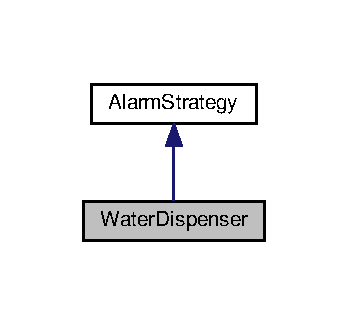
\includegraphics[width=167pt]{classWaterDispenser__coll__graph}
\end{center}
\end{figure}
\subsection*{Additional Inherited Members}


\subsection{Detailed Description}
Call firemen strategy class. 

Dummy implementation of call firemen strategy. Intended for testing purposes. 

The documentation for this class was generated from the following files\+:\begin{DoxyCompactItemize}
\item 
alarm-\/strategy/\hyperlink{waterdispenser_8h}{waterdispenser.\+h}\item 
alarm-\/strategy/\hyperlink{waterdispenser_8cpp}{waterdispenser.\+cpp}\end{DoxyCompactItemize}

\chapter{File Documentation}
\hypertarget{alarmcomponent_8cpp}{}\section{alarm-\/composite/alarmcomponent.cpp File Reference}
\label{alarmcomponent_8cpp}\index{alarm-\/composite/alarmcomponent.\+cpp@{alarm-\/composite/alarmcomponent.\+cpp}}
{\ttfamily \#include \char`\"{}alarmcomponent.\+h\char`\"{}}\\*
Include dependency graph for alarmcomponent.\+cpp\+:\nopagebreak
\begin{figure}[H]
\begin{center}
\leavevmode
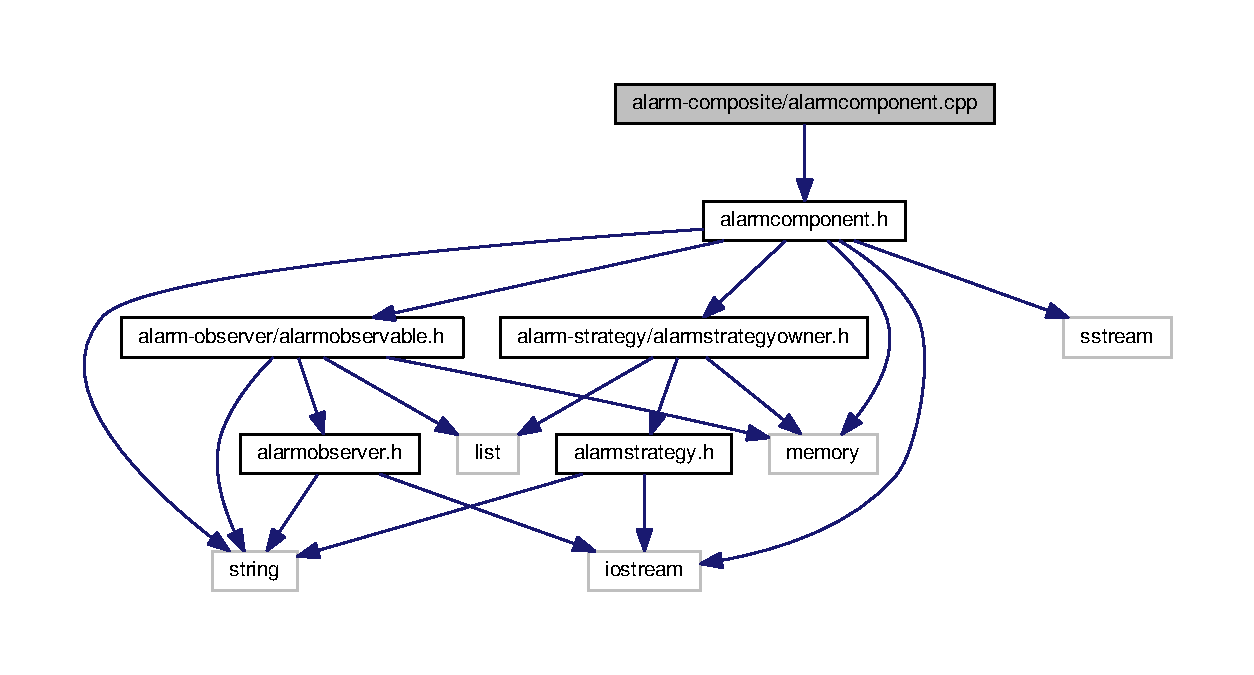
\includegraphics[width=350pt]{alarmcomponent_8cpp__incl}
\end{center}
\end{figure}


\subsection{Detailed Description}
\hyperlink{classAlarmComponent}{Alarm\+Component} class definition

\begin{DoxyVersion}{Version}
1.\+0
\end{DoxyVersion}
\begin{DoxyAuthor}{Author}
Vladimir Poliakov 

Brian Segers 
\end{DoxyAuthor}

\hypertarget{alarmcomponent_8h}{}\section{alarm-\/composite/alarmcomponent.h File Reference}
\label{alarmcomponent_8h}\index{alarm-\/composite/alarmcomponent.\+h@{alarm-\/composite/alarmcomponent.\+h}}
{\ttfamily \#include $<$string$>$}\\*
{\ttfamily \#include $<$iostream$>$}\\*
{\ttfamily \#include $<$memory$>$}\\*
{\ttfamily \#include $<$sstream$>$}\\*
{\ttfamily \#include \char`\"{}alarm-\/observer/alarmobservable.\+h\char`\"{}}\\*
Include dependency graph for alarmcomponent.\+h\+:\nopagebreak
\begin{figure}[H]
\begin{center}
\leavevmode
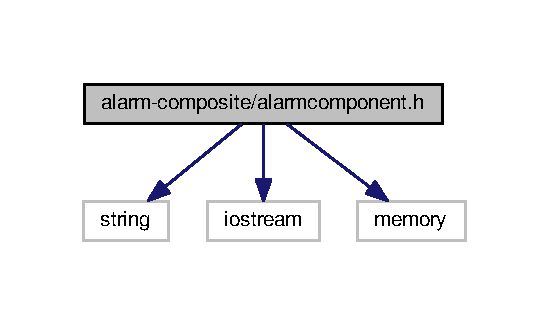
\includegraphics[width=350pt]{alarmcomponent_8h__incl}
\end{center}
\end{figure}
This graph shows which files directly or indirectly include this file\+:\nopagebreak
\begin{figure}[H]
\begin{center}
\leavevmode
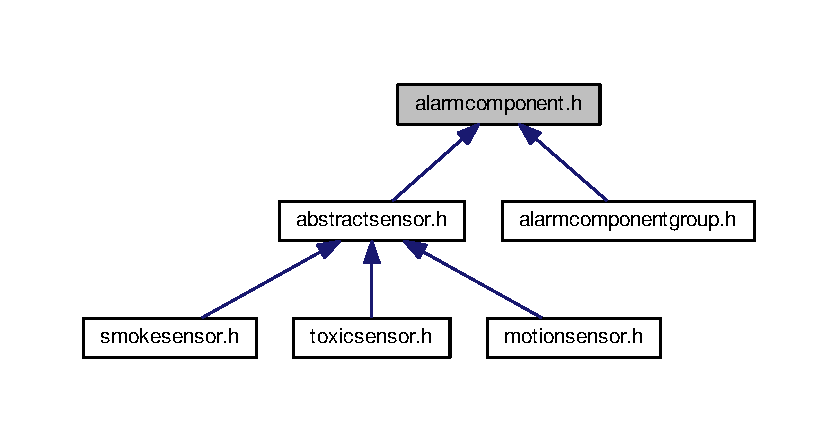
\includegraphics[width=350pt]{alarmcomponent_8h__dep__incl}
\end{center}
\end{figure}
\subsection*{Classes}
\begin{DoxyCompactItemize}
\item 
class \hyperlink{classAlarmComponent}{Alarm\+Component}
\begin{DoxyCompactList}\small\item\em Base component class of composite structure. \end{DoxyCompactList}\end{DoxyCompactItemize}


\subsection{Detailed Description}
\hyperlink{classAlarmComponent}{Alarm\+Component} class declaration

\begin{DoxyVersion}{Version}
1.\+0
\end{DoxyVersion}
\begin{DoxyAuthor}{Author}
Vladimir Poliakov 

Brian Segers 
\end{DoxyAuthor}

\hypertarget{alarmcomponentgroup_8cpp}{}\section{alarm-\/composite/alarmcomponentgroup.cpp File Reference}
\label{alarmcomponentgroup_8cpp}\index{alarm-\/composite/alarmcomponentgroup.\+cpp@{alarm-\/composite/alarmcomponentgroup.\+cpp}}
{\ttfamily \#include \char`\"{}alarmcomponentgroup.\+h\char`\"{}}\\*
Include dependency graph for alarmcomponentgroup.\+cpp\+:\nopagebreak
\begin{figure}[H]
\begin{center}
\leavevmode
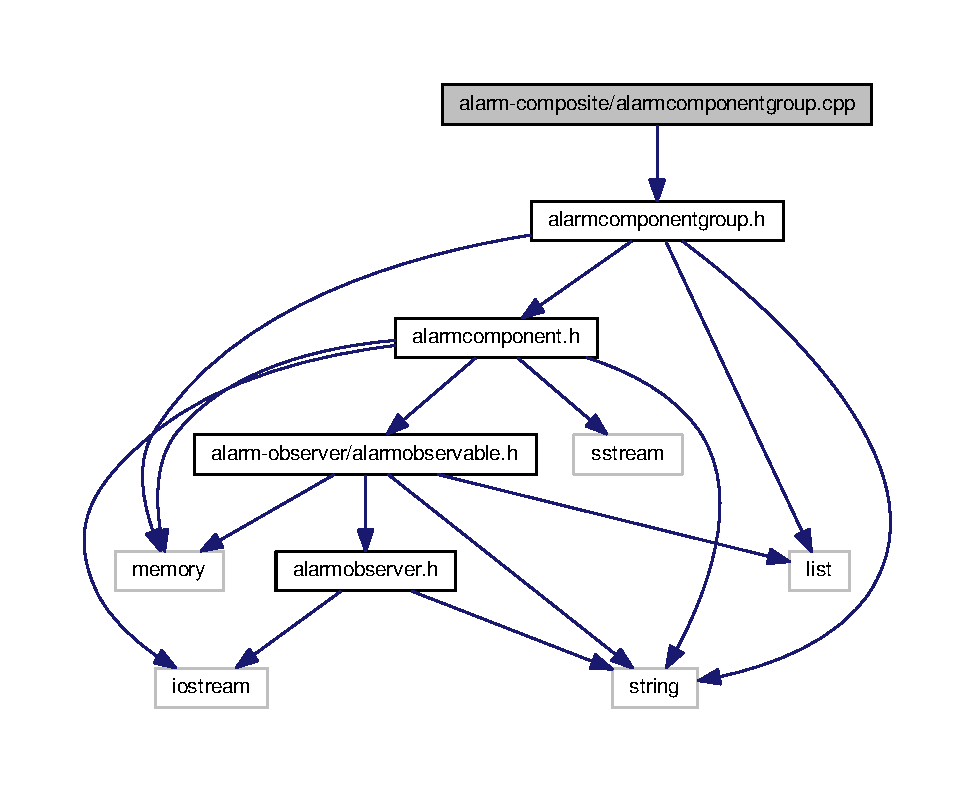
\includegraphics[width=350pt]{alarmcomponentgroup_8cpp__incl}
\end{center}
\end{figure}


\subsection{Detailed Description}
\hyperlink{classAlarmComponentGroup}{Alarm\+Component\+Group} class definition

\begin{DoxyVersion}{Version}
1.\+0
\end{DoxyVersion}
\begin{DoxyAuthor}{Author}
Vladimir Poliakov 

Brian Segers 
\end{DoxyAuthor}

\hypertarget{alarmcomponentgroup_8h}{}\section{alarm-\/composite/alarmcomponentgroup.h File Reference}
\label{alarmcomponentgroup_8h}\index{alarm-\/composite/alarmcomponentgroup.\+h@{alarm-\/composite/alarmcomponentgroup.\+h}}
{\ttfamily \#include $<$memory$>$}\\*
{\ttfamily \#include $<$string$>$}\\*
{\ttfamily \#include $<$list$>$}\\*
{\ttfamily \#include \char`\"{}alarmcomponent.\+h\char`\"{}}\\*
Include dependency graph for alarmcomponentgroup.\+h\+:\nopagebreak
\begin{figure}[H]
\begin{center}
\leavevmode
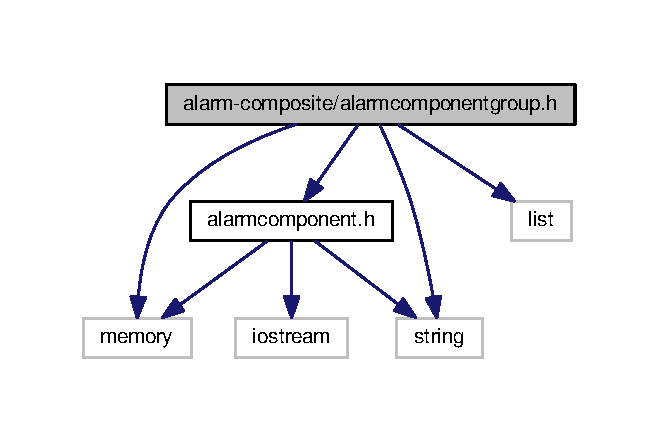
\includegraphics[width=350pt]{alarmcomponentgroup_8h__incl}
\end{center}
\end{figure}
This graph shows which files directly or indirectly include this file\+:\nopagebreak
\begin{figure}[H]
\begin{center}
\leavevmode
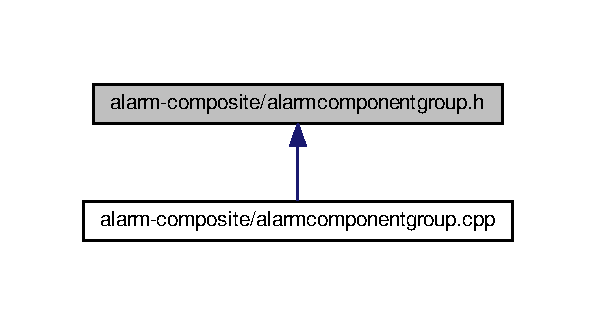
\includegraphics[width=286pt]{alarmcomponentgroup_8h__dep__incl}
\end{center}
\end{figure}
\subsection*{Classes}
\begin{DoxyCompactItemize}
\item 
class \hyperlink{classAlarmComponentGroup}{Alarm\+Component\+Group}
\begin{DoxyCompactList}\small\item\em Group component class of composite structure. \end{DoxyCompactList}\end{DoxyCompactItemize}


\subsection{Detailed Description}
\hyperlink{classAlarmComponentGroup}{Alarm\+Component\+Group} class declaration

\begin{DoxyVersion}{Version}
1.\+0
\end{DoxyVersion}
\begin{DoxyAuthor}{Author}
Vladimir Poliakov 

Brian Segers 
\end{DoxyAuthor}

\hypertarget{alarmobservable_8cpp}{}\section{alarm-\/observer/alarmobservable.cpp File Reference}
\label{alarmobservable_8cpp}\index{alarm-\/observer/alarmobservable.\+cpp@{alarm-\/observer/alarmobservable.\+cpp}}
{\ttfamily \#include \char`\"{}alarmobservable.\+h\char`\"{}}\\*
Include dependency graph for alarmobservable.\+cpp\+:\nopagebreak
\begin{figure}[H]
\begin{center}
\leavevmode
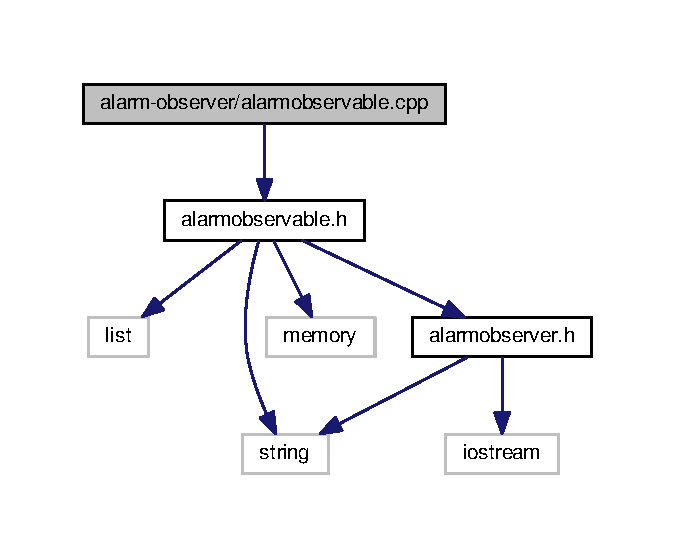
\includegraphics[width=324pt]{alarmobservable_8cpp__incl}
\end{center}
\end{figure}


\subsection{Detailed Description}
\hyperlink{classAlarmObservable}{Alarm\+Observable} class definition

\begin{DoxyVersion}{Version}
1.\+0
\end{DoxyVersion}
\begin{DoxyAuthor}{Author}
Vladimir Poliakov 

Brian Segers 
\end{DoxyAuthor}

\hypertarget{alarmobservable_8h}{}\section{alarm-\/observer/alarmobservable.h File Reference}
\label{alarmobservable_8h}\index{alarm-\/observer/alarmobservable.\+h@{alarm-\/observer/alarmobservable.\+h}}
{\ttfamily \#include $<$list$>$}\\*
{\ttfamily \#include $<$string$>$}\\*
{\ttfamily \#include $<$memory$>$}\\*
{\ttfamily \#include \char`\"{}alarmobserver.\+h\char`\"{}}\\*
Include dependency graph for alarmobservable.\+h\+:\nopagebreak
\begin{figure}[H]
\begin{center}
\leavevmode
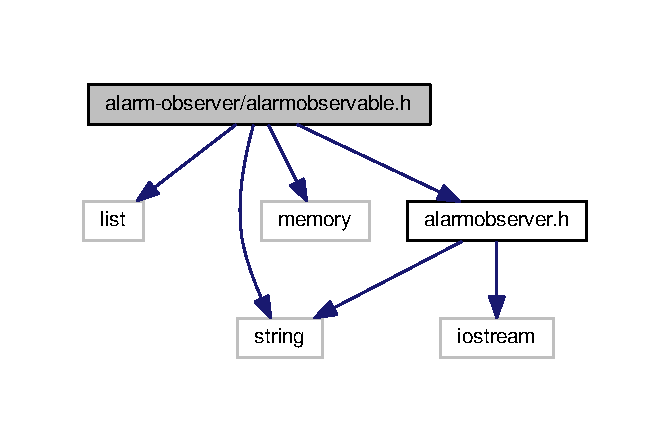
\includegraphics[width=322pt]{alarmobservable_8h__incl}
\end{center}
\end{figure}
This graph shows which files directly or indirectly include this file\+:\nopagebreak
\begin{figure}[H]
\begin{center}
\leavevmode
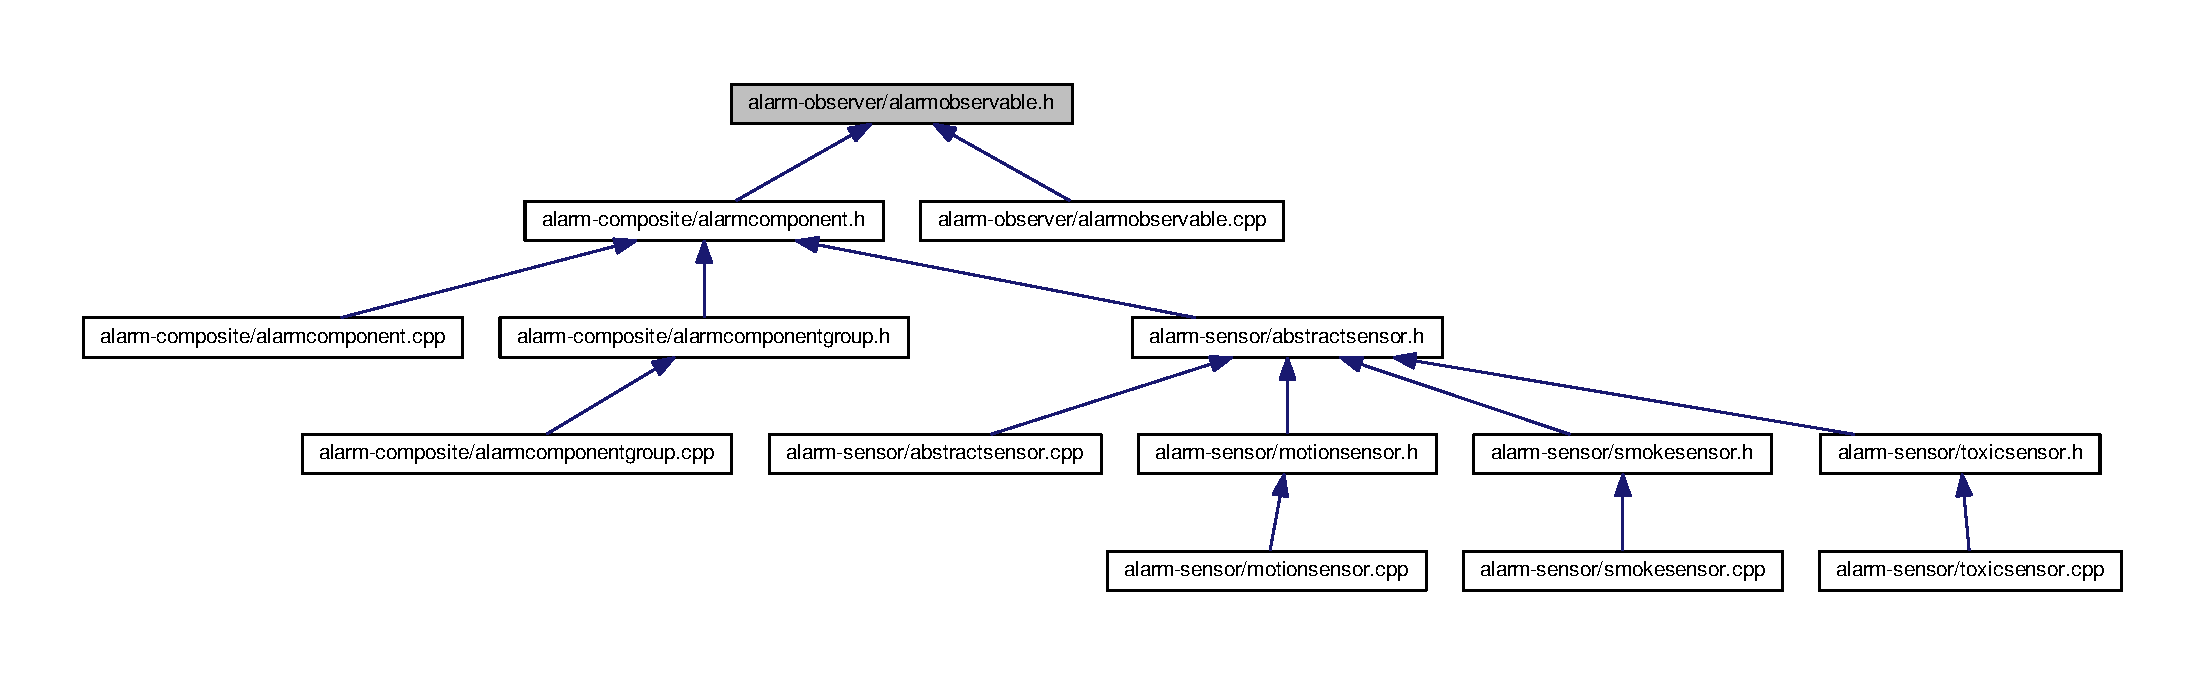
\includegraphics[width=350pt]{alarmobservable_8h__dep__incl}
\end{center}
\end{figure}
\subsection*{Classes}
\begin{DoxyCompactItemize}
\item 
class \hyperlink{classAlarmObservable}{Alarm\+Observable}
\begin{DoxyCompactList}\small\item\em Observable class of observer structure. \end{DoxyCompactList}\end{DoxyCompactItemize}


\subsection{Detailed Description}
\hyperlink{classAlarmObservable}{Alarm\+Observable} class declaration

\begin{DoxyVersion}{Version}
1.\+0
\end{DoxyVersion}
\begin{DoxyAuthor}{Author}
Vladimir Poliakov 

Brian Segers 
\end{DoxyAuthor}

\hypertarget{alarmobserver_8cpp}{}\section{alarm-\/observer/alarmobserver.cpp File Reference}
\label{alarmobserver_8cpp}\index{alarm-\/observer/alarmobserver.\+cpp@{alarm-\/observer/alarmobserver.\+cpp}}
{\ttfamily \#include \char`\"{}alarmobserver.\+h\char`\"{}}\\*
Include dependency graph for alarmobserver.\+cpp\+:\nopagebreak
\begin{figure}[H]
\begin{center}
\leavevmode
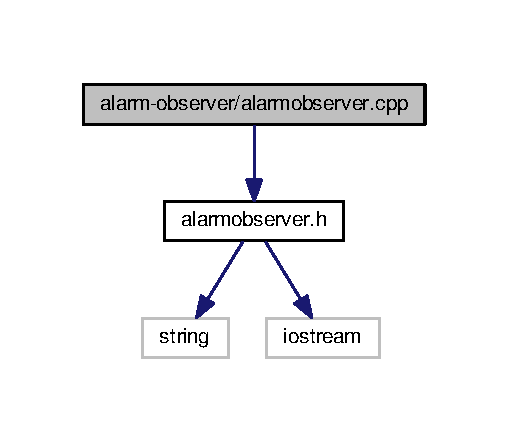
\includegraphics[width=244pt]{alarmobserver_8cpp__incl}
\end{center}
\end{figure}


\subsection{Detailed Description}
\hyperlink{classAlarmObserver}{Alarm\+Observer} class definition

\begin{DoxyVersion}{Version}
1.\+0
\end{DoxyVersion}
\begin{DoxyAuthor}{Author}
Vladimir Poliakov 

Brian Segers 
\end{DoxyAuthor}

\hypertarget{alarmobserver_8h}{}\section{alarm-\/observer/alarmobserver.h File Reference}
\label{alarmobserver_8h}\index{alarm-\/observer/alarmobserver.\+h@{alarm-\/observer/alarmobserver.\+h}}
{\ttfamily \#include $<$string$>$}\\*
{\ttfamily \#include $<$iostream$>$}\\*
Include dependency graph for alarmobserver.\+h\+:\nopagebreak
\begin{figure}[H]
\begin{center}
\leavevmode
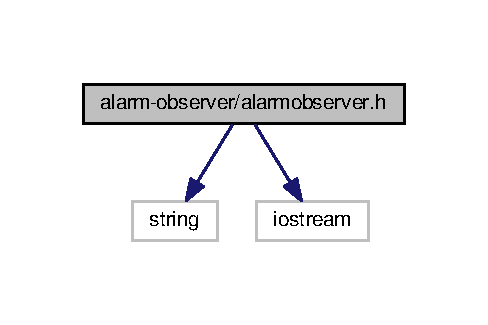
\includegraphics[width=234pt]{alarmobserver_8h__incl}
\end{center}
\end{figure}
This graph shows which files directly or indirectly include this file\+:\nopagebreak
\begin{figure}[H]
\begin{center}
\leavevmode
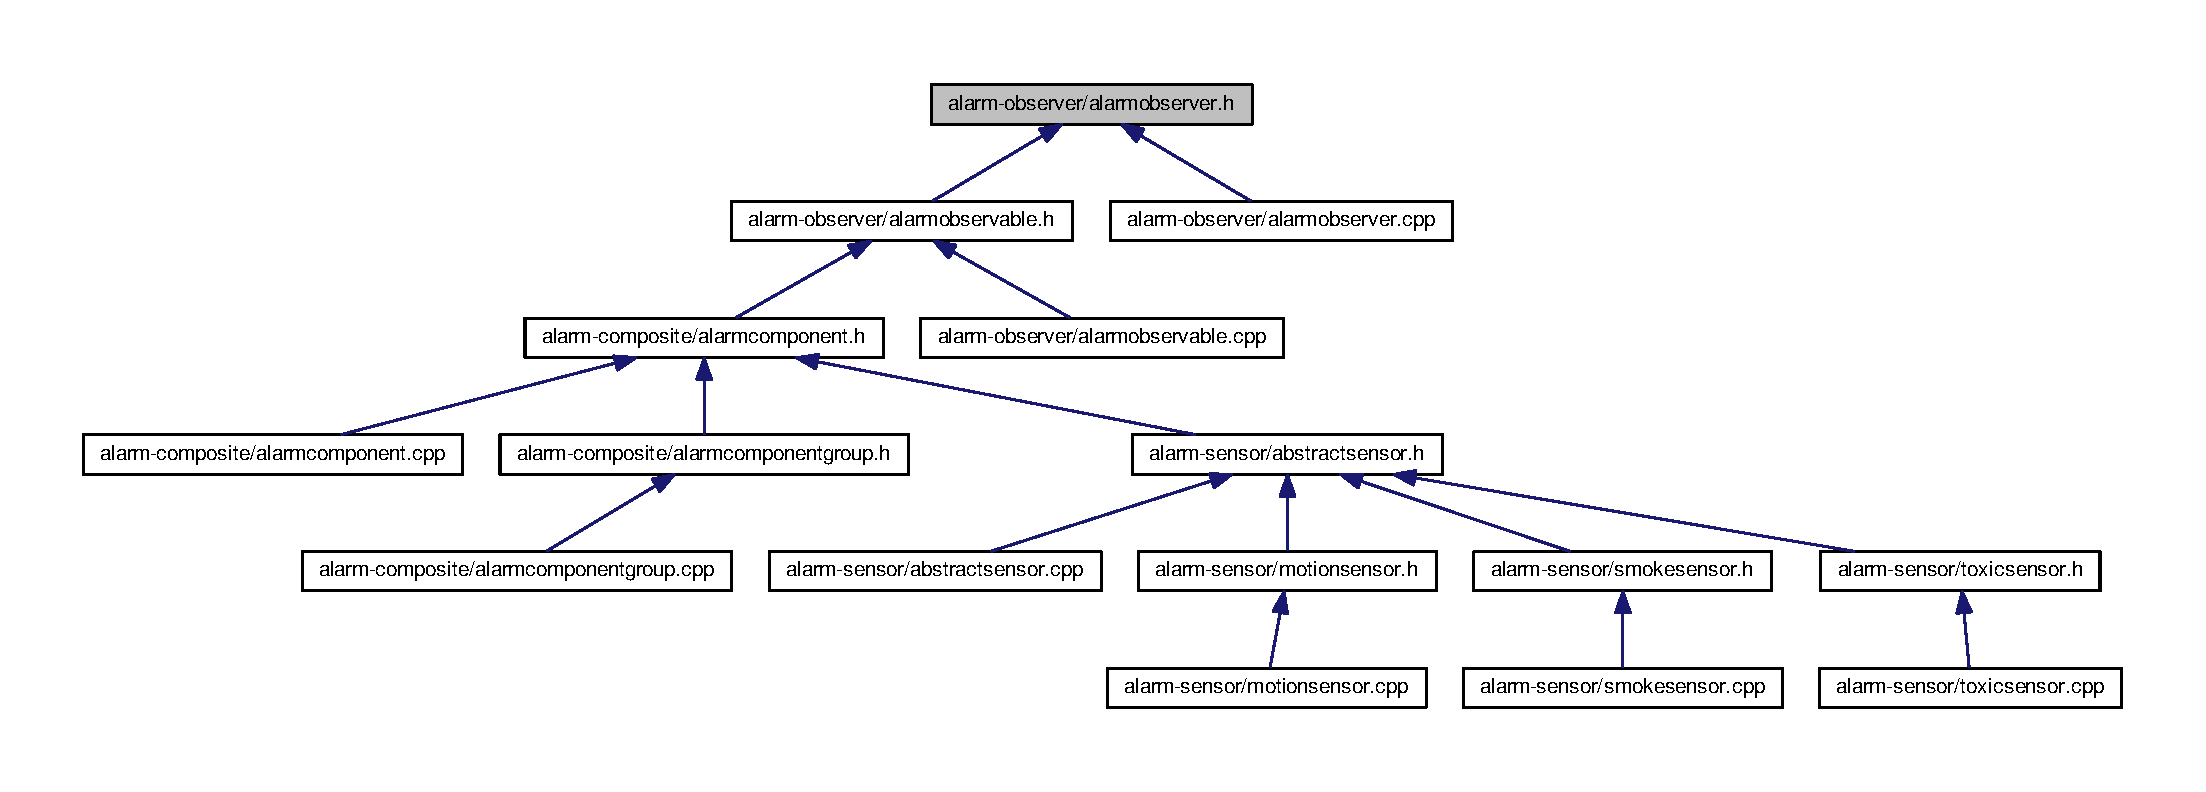
\includegraphics[width=350pt]{alarmobserver_8h__dep__incl}
\end{center}
\end{figure}
\subsection*{Classes}
\begin{DoxyCompactItemize}
\item 
class \hyperlink{classAlarmObserver}{Alarm\+Observer}
\begin{DoxyCompactList}\small\item\em Observer class of observer structure. \end{DoxyCompactList}\end{DoxyCompactItemize}


\subsection{Detailed Description}
\hyperlink{classAlarmObserver}{Alarm\+Observer} class declaration

\begin{DoxyVersion}{Version}
1.\+0
\end{DoxyVersion}
\begin{DoxyAuthor}{Author}
Vladimir Poliakov 

Brian Segers 
\end{DoxyAuthor}

\hypertarget{abstractsensor_8cpp}{}\section{alarm-\/sensor/abstractsensor.cpp File Reference}
\label{abstractsensor_8cpp}\index{alarm-\/sensor/abstractsensor.\+cpp@{alarm-\/sensor/abstractsensor.\+cpp}}
{\ttfamily \#include \char`\"{}abstractsensor.\+h\char`\"{}}\\*
Include dependency graph for abstractsensor.\+cpp\+:\nopagebreak
\begin{figure}[H]
\begin{center}
\leavevmode
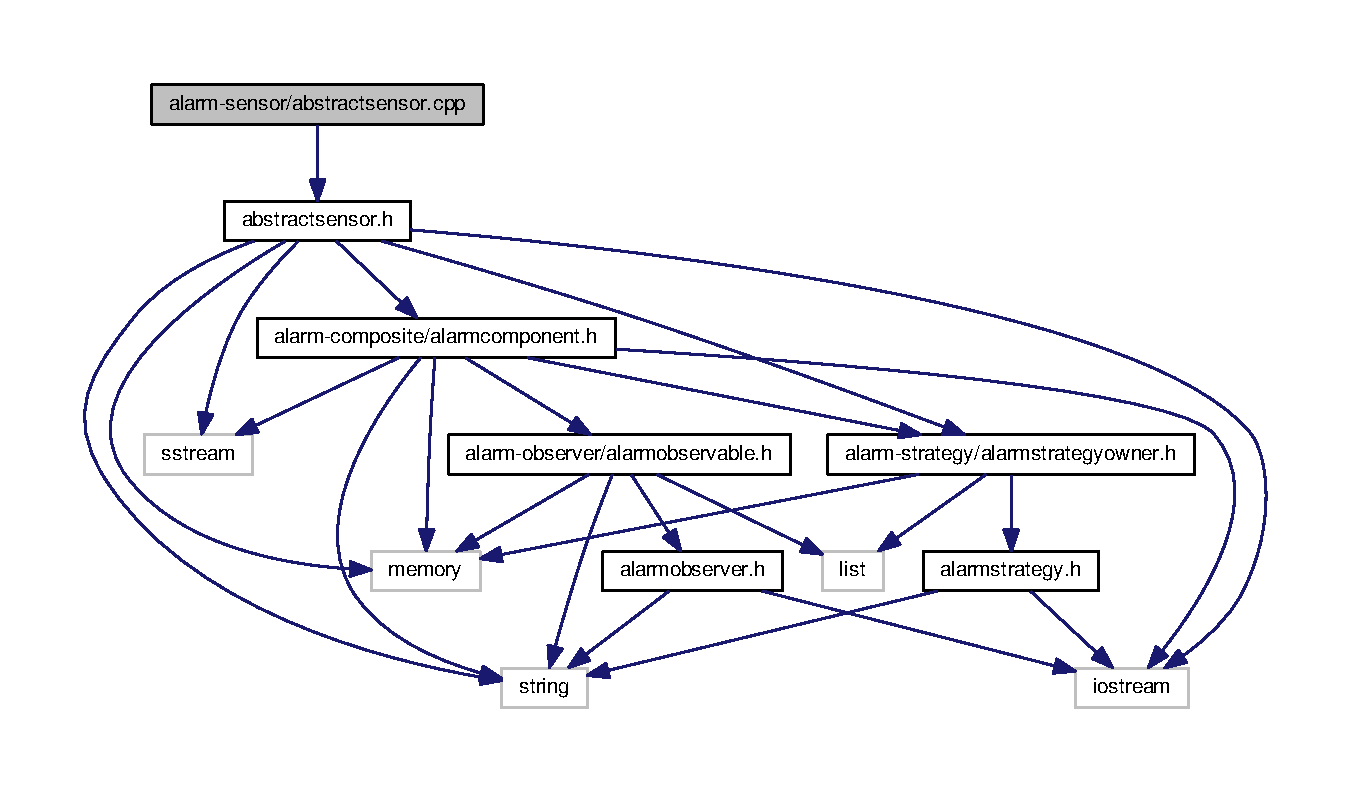
\includegraphics[width=350pt]{abstractsensor_8cpp__incl}
\end{center}
\end{figure}
\subsection*{Functions}
\begin{DoxyCompactItemize}
\item 
ostream \& {\bfseries operator$<$$<$} (ostream \&lhs, const shared\+\_\+ptr$<$ \hyperlink{classAbstractSensor}{Abstract\+Sensor} $>$ \&rhs)\hypertarget{abstractsensor_8cpp_a576af0723bfc4c3f2d57ad44e4daec59}{}\label{abstractsensor_8cpp_a576af0723bfc4c3f2d57ad44e4daec59}

\end{DoxyCompactItemize}


\subsection{Detailed Description}
\hyperlink{classAbstractSensor}{Abstract\+Sensor} class definition

\begin{DoxyVersion}{Version}
1.\+0
\end{DoxyVersion}
\begin{DoxyAuthor}{Author}
Vladimir Poliakov 

Brian Segers 
\end{DoxyAuthor}

\hypertarget{abstractsensor_8h}{}\section{alarm-\/sensor/abstractsensor.h File Reference}
\label{abstractsensor_8h}\index{alarm-\/sensor/abstractsensor.\+h@{alarm-\/sensor/abstractsensor.\+h}}
{\ttfamily \#include $<$iostream$>$}\\*
{\ttfamily \#include $<$string$>$}\\*
{\ttfamily \#include $<$memory$>$}\\*
{\ttfamily \#include $<$sstream$>$}\\*
{\ttfamily \#include \char`\"{}alarm-\/composite/alarmcomponent.\+h\char`\"{}}\\*
{\ttfamily \#include \char`\"{}alarm-\/strategy/alarmstrategyowner.\+h\char`\"{}}\\*
Include dependency graph for abstractsensor.\+h\+:\nopagebreak
\begin{figure}[H]
\begin{center}
\leavevmode
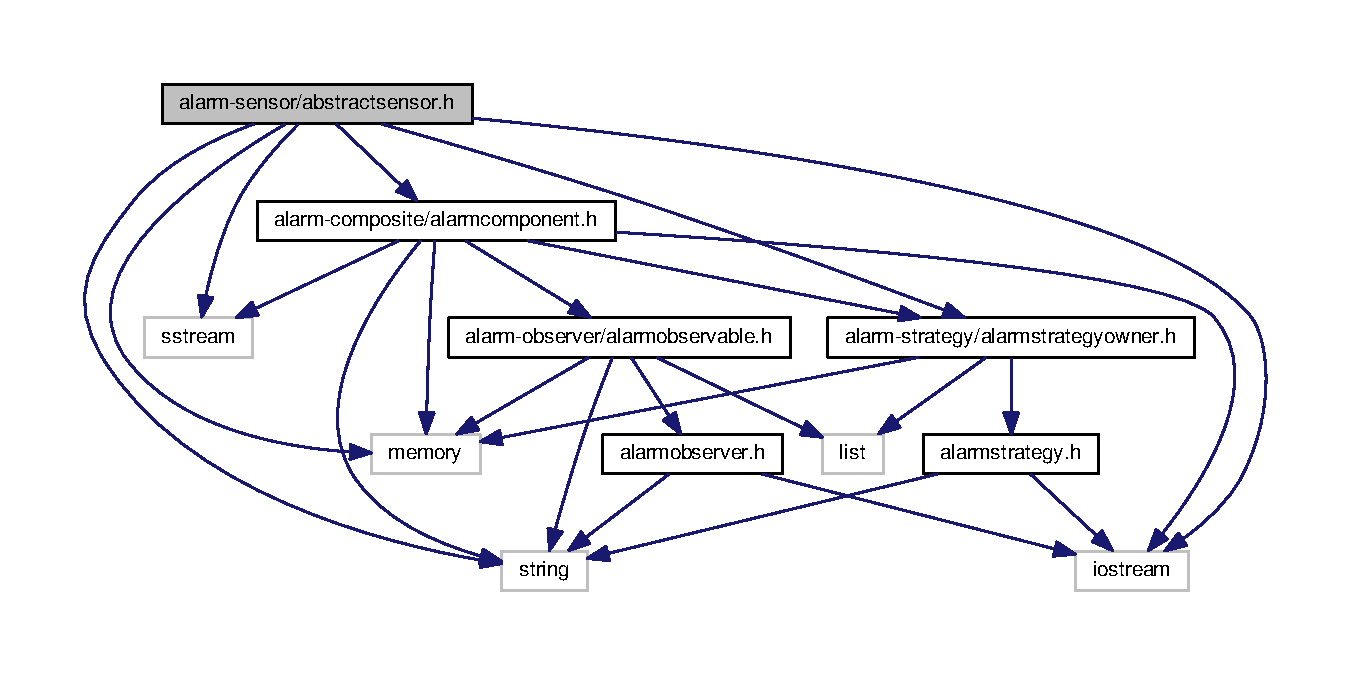
\includegraphics[width=350pt]{abstractsensor_8h__incl}
\end{center}
\end{figure}
This graph shows which files directly or indirectly include this file\+:\nopagebreak
\begin{figure}[H]
\begin{center}
\leavevmode
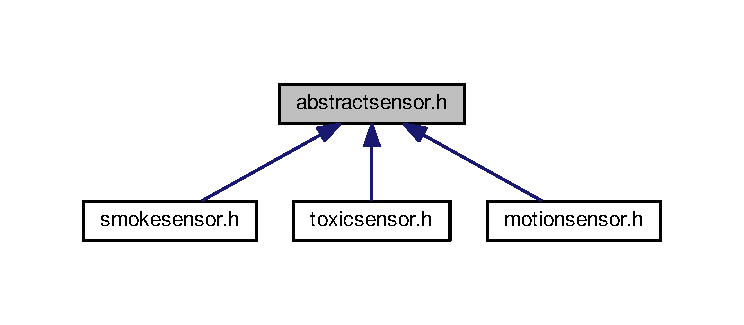
\includegraphics[width=350pt]{abstractsensor_8h__dep__incl}
\end{center}
\end{figure}
\subsection*{Classes}
\begin{DoxyCompactItemize}
\item 
class \hyperlink{classAbstractSensor}{Abstract\+Sensor}
\begin{DoxyCompactList}\small\item\em Abstract sensor class. \end{DoxyCompactList}\item 
class \hyperlink{classcompareByVendor}{compare\+By\+Vendor}
\begin{DoxyCompactList}\small\item\em Sorting by vendor functor for Alarm\+Sensors. \end{DoxyCompactList}\item 
class \hyperlink{classcompareByType}{compare\+By\+Type}
\begin{DoxyCompactList}\small\item\em Sorting by type functor for Alarm\+Sensors. \end{DoxyCompactList}\item 
class \hyperlink{classcompareByVendorByType}{compare\+By\+Vendor\+By\+Type}
\begin{DoxyCompactList}\small\item\em Sorting by vendor by type functor for Alarm\+Sensors. \end{DoxyCompactList}\end{DoxyCompactItemize}
\subsection*{Functions}
\begin{DoxyCompactItemize}
\item 
const std\+::shared\+\_\+ptr$<$ \hyperlink{classAbstractSensor}{Abstract\+Sensor} $>$ \& \hyperlink{abstractsensor_8h_a7edf3477b3c13417667c4a6435df15c9}{operator++} (const std\+::shared\+\_\+ptr$<$ \hyperlink{classAbstractSensor}{Abstract\+Sensor} $>$ \&rhs)
\begin{DoxyCompactList}\small\item\em Same as \hyperlink{classAlarmComponent_ab2acf6b580efe04bd617580ecb7323f1}{Abstract\+Sensor\+::activate()} \end{DoxyCompactList}\item 
const std\+::shared\+\_\+ptr$<$ \hyperlink{classAbstractSensor}{Abstract\+Sensor} $>$ \& \hyperlink{abstractsensor_8h_aae41e9a8ba67cf08df99026539a54211}{operator-\/-\/} (const std\+::shared\+\_\+ptr$<$ \hyperlink{classAbstractSensor}{Abstract\+Sensor} $>$ \&rhs)
\begin{DoxyCompactList}\small\item\em Same as \hyperlink{classAlarmComponent_aef44069a068e92ccd15b3afcbd06dff6}{Abstract\+Sensor\+::deactivate()} \end{DoxyCompactList}\item 
std\+::ostream \& \hyperlink{abstractsensor_8h_a3cf071ea4ace6fbefd044549ac80b476}{operator$<$$<$} (std\+::ostream \&lhs, const std\+::shared\+\_\+ptr$<$ \hyperlink{classAbstractSensor}{Abstract\+Sensor} $>$ \&rhs)
\begin{DoxyCompactList}\small\item\em Passes info about the sensor to the output stream. \end{DoxyCompactList}\end{DoxyCompactItemize}


\subsection{Detailed Description}
\hyperlink{classAbstractSensor}{Abstract\+Sensor} class declaration

\begin{DoxyVersion}{Version}
1.\+0
\end{DoxyVersion}
\begin{DoxyAuthor}{Author}
Vladimir Poliakov 

Brian Segers 
\end{DoxyAuthor}


\subsection{Function Documentation}
\index{abstractsensor.\+h@{abstractsensor.\+h}!operator++@{operator++}}
\index{operator++@{operator++}!abstractsensor.\+h@{abstractsensor.\+h}}
\subsubsection[{\texorpdfstring{operator++(const std\+::shared\+\_\+ptr$<$ Abstract\+Sensor $>$ \&rhs)}{operator++(const std::shared_ptr< AbstractSensor > &rhs)}}]{\setlength{\rightskip}{0pt plus 5cm}const std\+::shared\+\_\+ptr$<${\bf Abstract\+Sensor}$>$\& operator++ (
\begin{DoxyParamCaption}
\item[{const std\+::shared\+\_\+ptr$<$ {\bf Abstract\+Sensor} $>$ \&}]{rhs}
\end{DoxyParamCaption}
)\hspace{0.3cm}{\ttfamily [inline]}}\hypertarget{abstractsensor_8h_a7edf3477b3c13417667c4a6435df15c9}{}\label{abstractsensor_8h_a7edf3477b3c13417667c4a6435df15c9}


Same as \hyperlink{classAlarmComponent_ab2acf6b580efe04bd617580ecb7323f1}{Abstract\+Sensor\+::activate()} 

\begin{DoxyNote}{Note}
This is an overloaded function 
\end{DoxyNote}
\index{abstractsensor.\+h@{abstractsensor.\+h}!operator-\/-\/@{operator-\/-\/}}
\index{operator-\/-\/@{operator-\/-\/}!abstractsensor.\+h@{abstractsensor.\+h}}
\subsubsection[{\texorpdfstring{operator-\/-\/(const std\+::shared\+\_\+ptr$<$ Abstract\+Sensor $>$ \&rhs)}{operator--(const std::shared_ptr< AbstractSensor > &rhs)}}]{\setlength{\rightskip}{0pt plus 5cm}const std\+::shared\+\_\+ptr$<${\bf Abstract\+Sensor}$>$\& operator-\/-\/ (
\begin{DoxyParamCaption}
\item[{const std\+::shared\+\_\+ptr$<$ {\bf Abstract\+Sensor} $>$ \&}]{rhs}
\end{DoxyParamCaption}
)\hspace{0.3cm}{\ttfamily [inline]}}\hypertarget{abstractsensor_8h_aae41e9a8ba67cf08df99026539a54211}{}\label{abstractsensor_8h_aae41e9a8ba67cf08df99026539a54211}


Same as \hyperlink{classAlarmComponent_aef44069a068e92ccd15b3afcbd06dff6}{Abstract\+Sensor\+::deactivate()} 

\begin{DoxyNote}{Note}
This is an overloaded function 
\end{DoxyNote}
\index{abstractsensor.\+h@{abstractsensor.\+h}!operator$<$$<$@{operator$<$$<$}}
\index{operator$<$$<$@{operator$<$$<$}!abstractsensor.\+h@{abstractsensor.\+h}}
\subsubsection[{\texorpdfstring{operator$<$$<$(std\+::ostream \&lhs, const std\+::shared\+\_\+ptr$<$ Abstract\+Sensor $>$ \&rhs)}{operator<<(std::ostream &lhs, const std::shared_ptr< AbstractSensor > &rhs)}}]{\setlength{\rightskip}{0pt plus 5cm}std\+::ostream\& operator$<$$<$ (
\begin{DoxyParamCaption}
\item[{std\+::ostream \&}]{lhs, }
\item[{const std\+::shared\+\_\+ptr$<$ {\bf Abstract\+Sensor} $>$ \&}]{rhs}
\end{DoxyParamCaption}
)}\hypertarget{abstractsensor_8h_a3cf071ea4ace6fbefd044549ac80b476}{}\label{abstractsensor_8h_a3cf071ea4ace6fbefd044549ac80b476}


Passes info about the sensor to the output stream. 

\begin{DoxyNote}{Note}
This is an overloaded function 
\end{DoxyNote}

\hypertarget{motionsensor_8cpp}{}\section{alarm-\/sensor/motionsensor.cpp File Reference}
\label{motionsensor_8cpp}\index{alarm-\/sensor/motionsensor.\+cpp@{alarm-\/sensor/motionsensor.\+cpp}}
{\ttfamily \#include \char`\"{}motionsensor.\+h\char`\"{}}\\*
Include dependency graph for motionsensor.\+cpp\+:\nopagebreak
\begin{figure}[H]
\begin{center}
\leavevmode
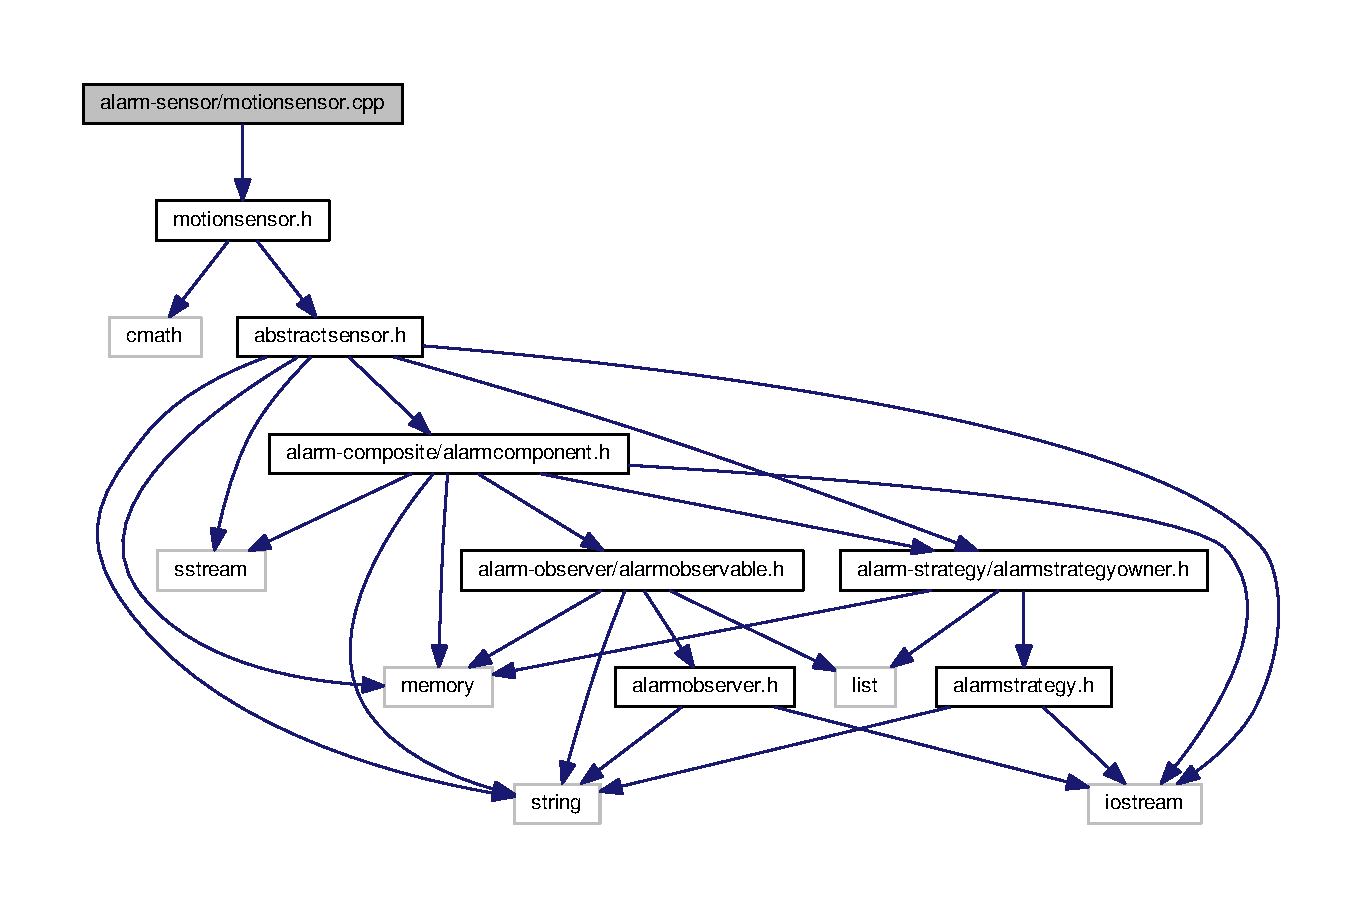
\includegraphics[width=350pt]{motionsensor_8cpp__incl}
\end{center}
\end{figure}


\subsection{Detailed Description}
\hyperlink{classMotionSensor}{Motion\+Sensor} class definition

\begin{DoxyVersion}{Version}
1.\+0
\end{DoxyVersion}
\begin{DoxyAuthor}{Author}
Vladimir Poliakov 

Brian Segers 
\end{DoxyAuthor}

\hypertarget{motionsensor_8h}{}\section{alarm-\/sensor/motionsensor.h File Reference}
\label{motionsensor_8h}\index{alarm-\/sensor/motionsensor.\+h@{alarm-\/sensor/motionsensor.\+h}}
{\ttfamily \#include $<$cmath$>$}\\*
{\ttfamily \#include \char`\"{}abstractsensor.\+h\char`\"{}}\\*
Include dependency graph for motionsensor.\+h\+:
\nopagebreak
\begin{figure}[H]
\begin{center}
\leavevmode
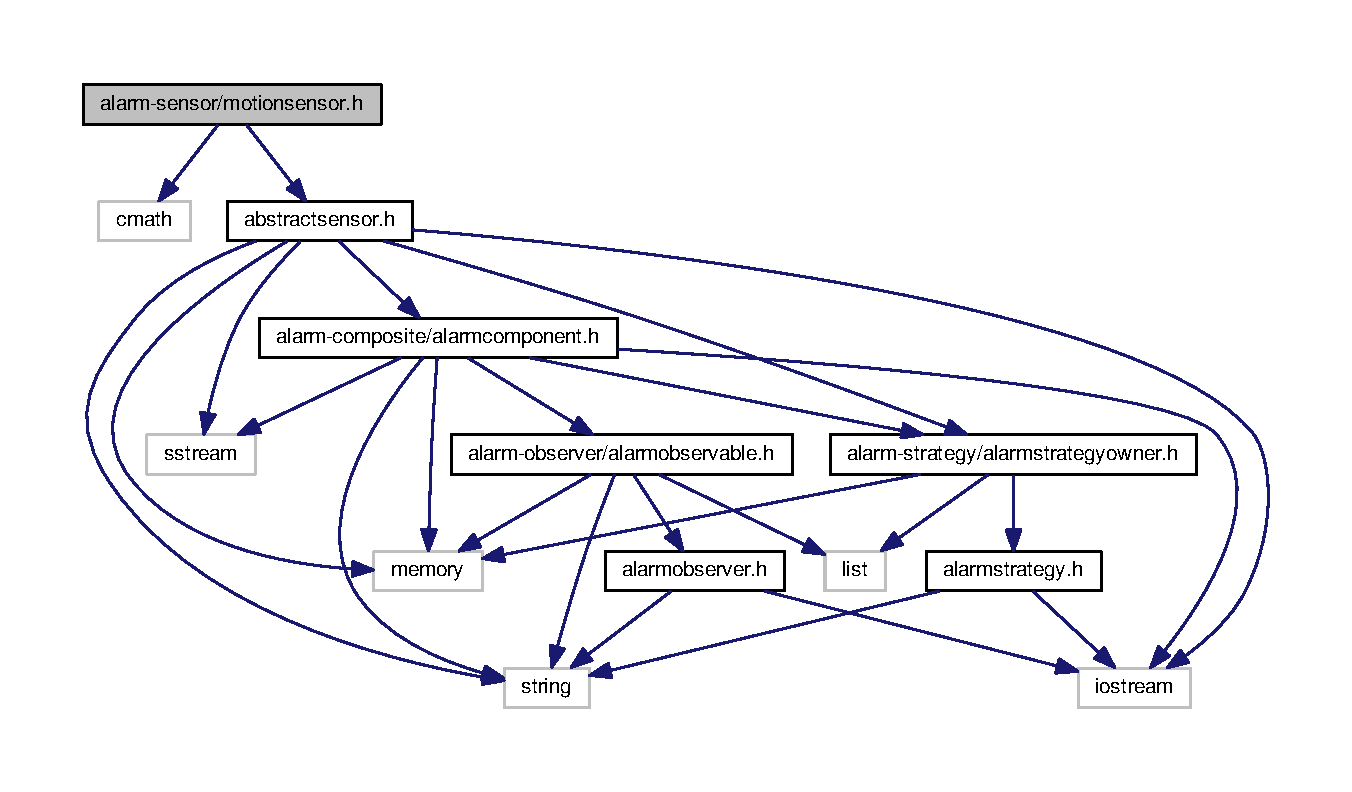
\includegraphics[width=350pt]{motionsensor_8h__incl}
\end{center}
\end{figure}
\subsection*{Classes}
\begin{DoxyCompactItemize}
\item 
class \hyperlink{classMotionSensor}{Motion\+Sensor}
\begin{DoxyCompactList}\small\item\em Motion sensor class. \end{DoxyCompactList}\end{DoxyCompactItemize}
\subsection*{Functions}
\begin{DoxyCompactItemize}
\item 
std\+::ostream \& \hyperlink{motionsensor_8h_a460a213e689a60bfd36d00b2dcf308c5}{operator$<$$<$} (std\+::ostream \&lhs, const std\+::shared\+\_\+ptr$<$ \hyperlink{classMotionSensor}{Motion\+Sensor} $>$ \&rhs)
\begin{DoxyCompactList}\small\item\em Passes info about the sensor to the output stream. \end{DoxyCompactList}\end{DoxyCompactItemize}


\subsection{Detailed Description}
\hyperlink{classMotionSensor}{Motion\+Sensor} class declaration

\begin{DoxyVersion}{Version}
1.\+0
\end{DoxyVersion}
\begin{DoxyAuthor}{Author}
Vladimir Poliakov 

Brian Segers 
\end{DoxyAuthor}


\subsection{Function Documentation}
\index{motionsensor.\+h@{motionsensor.\+h}!operator$<$$<$@{operator$<$$<$}}
\index{operator$<$$<$@{operator$<$$<$}!motionsensor.\+h@{motionsensor.\+h}}
\subsubsection[{\texorpdfstring{operator$<$$<$(std\+::ostream \&lhs, const std\+::shared\+\_\+ptr$<$ Motion\+Sensor $>$ \&rhs)}{operator<<(std::ostream &lhs, const std::shared_ptr< MotionSensor > &rhs)}}]{\setlength{\rightskip}{0pt plus 5cm}std\+::ostream\& operator$<$$<$ (
\begin{DoxyParamCaption}
\item[{std\+::ostream \&}]{lhs, }
\item[{const std\+::shared\+\_\+ptr$<$ {\bf Motion\+Sensor} $>$ \&}]{rhs}
\end{DoxyParamCaption}
)\hspace{0.3cm}{\ttfamily [inline]}}\hypertarget{motionsensor_8h_a460a213e689a60bfd36d00b2dcf308c5}{}\label{motionsensor_8h_a460a213e689a60bfd36d00b2dcf308c5}


Passes info about the sensor to the output stream. 

\begin{DoxyNote}{Note}
This is an overloaded function 
\end{DoxyNote}

\hypertarget{smokesensor_8cpp}{}\section{alarm-\/sensor/smokesensor.cpp File Reference}
\label{smokesensor_8cpp}\index{alarm-\/sensor/smokesensor.\+cpp@{alarm-\/sensor/smokesensor.\+cpp}}
{\ttfamily \#include \char`\"{}smokesensor.\+h\char`\"{}}\\*
Include dependency graph for smokesensor.\+cpp\+:\nopagebreak
\begin{figure}[H]
\begin{center}
\leavevmode
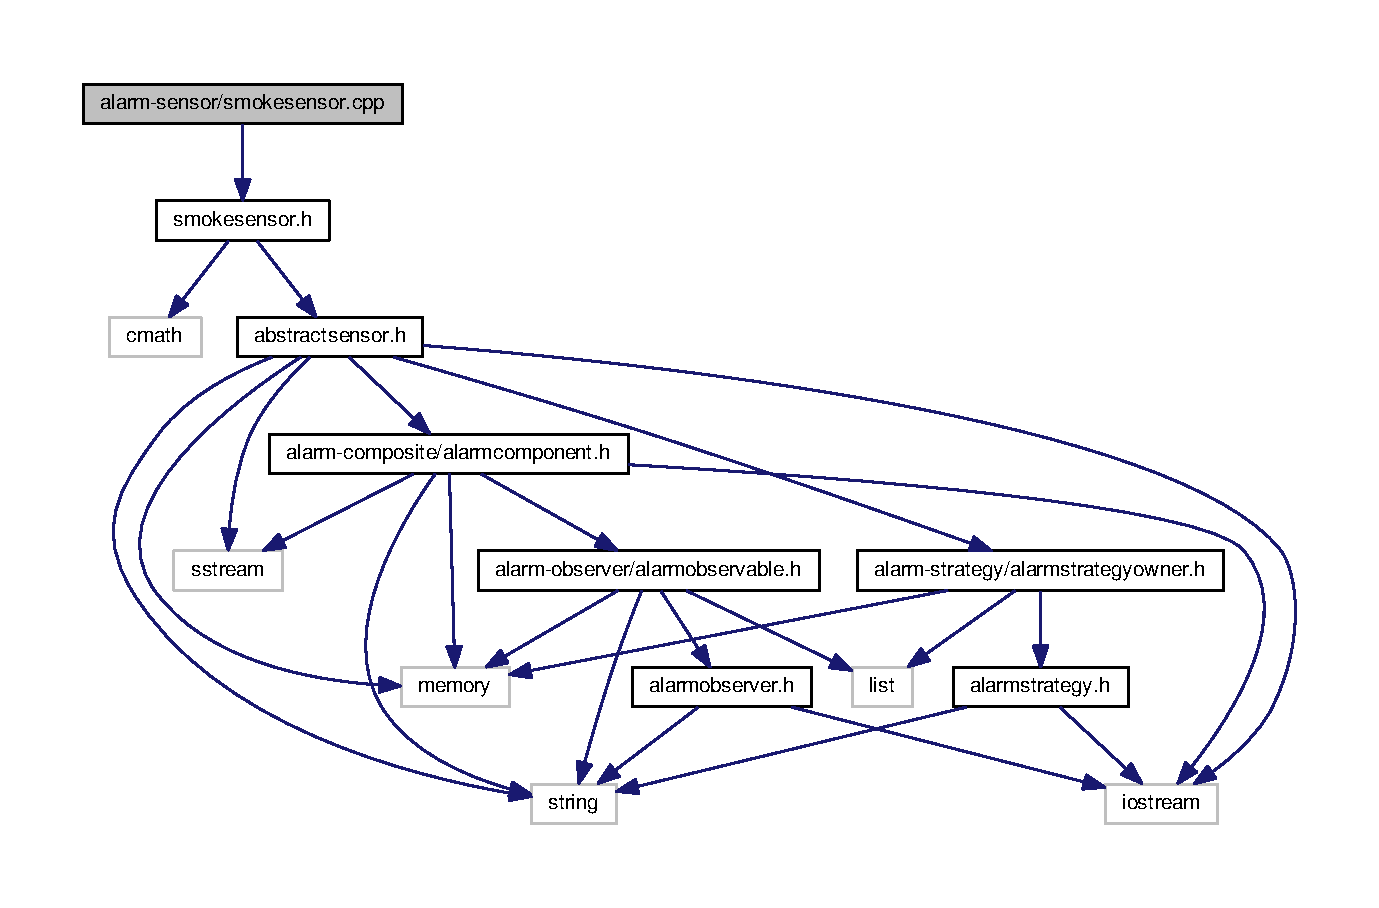
\includegraphics[width=350pt]{smokesensor_8cpp__incl}
\end{center}
\end{figure}


\subsection{Detailed Description}
\hyperlink{classSmokeSensor}{Smoke\+Sensor} class definition

\begin{DoxyVersion}{Version}
1.\+0
\end{DoxyVersion}
\begin{DoxyAuthor}{Author}
Vladimir Poliakov 

Brian Segers 
\end{DoxyAuthor}

\hypertarget{smokesensor_8h}{}\section{smokesensor.\+h File Reference}
\label{smokesensor_8h}\index{smokesensor.\+h@{smokesensor.\+h}}
{\ttfamily \#include $<$cmath$>$}\\*
{\ttfamily \#include $<$iostream$>$}\\*
{\ttfamily \#include $<$string$>$}\\*
{\ttfamily \#include \char`\"{}abstractsensor.\+h\char`\"{}}\\*
Include dependency graph for smokesensor.\+h\+:\nopagebreak
\begin{figure}[H]
\begin{center}
\leavevmode
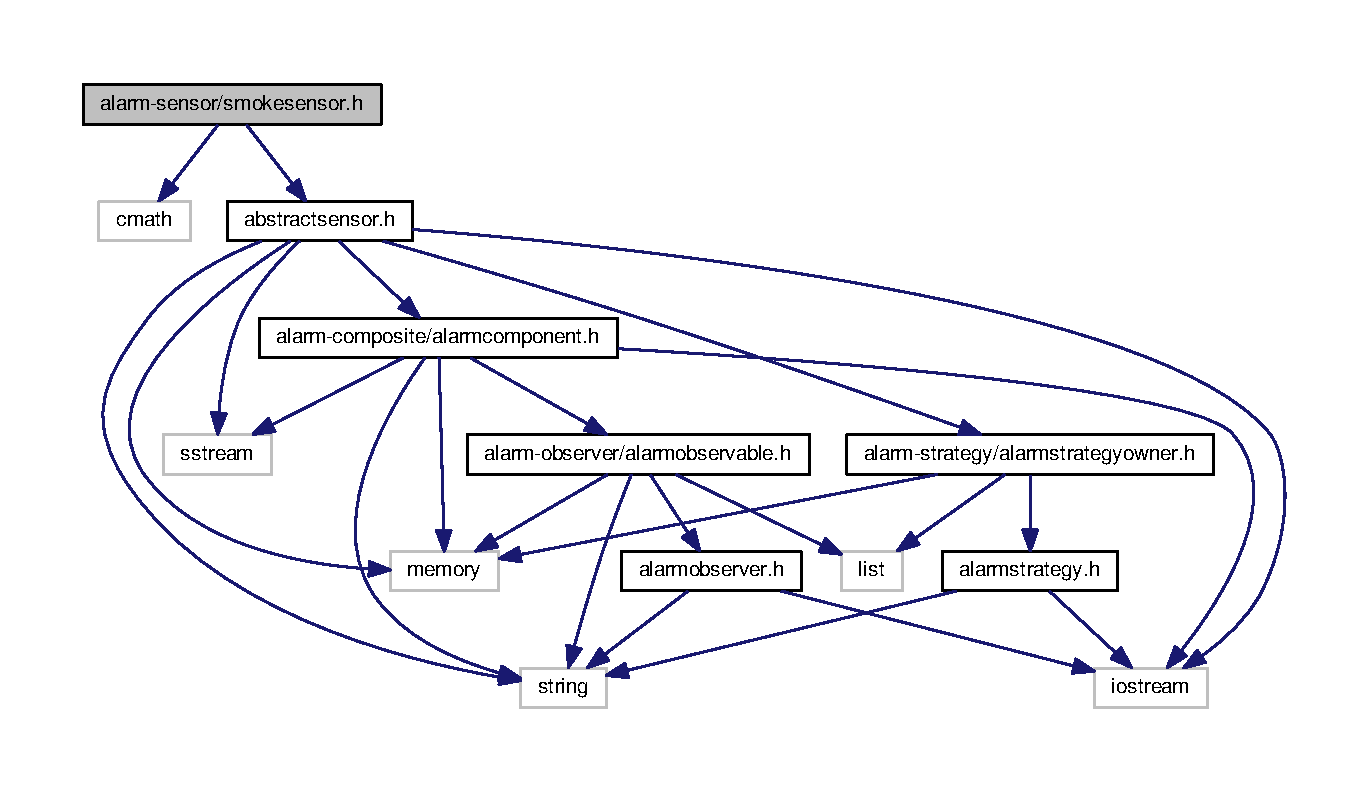
\includegraphics[width=350pt]{smokesensor_8h__incl}
\end{center}
\end{figure}
\subsection*{Classes}
\begin{DoxyCompactItemize}
\item 
class \hyperlink{classSmokeSensor}{Smoke\+Sensor}
\begin{DoxyCompactList}\small\item\em Smoke sensor class. \end{DoxyCompactList}\end{DoxyCompactItemize}


\subsection{Detailed Description}
\hyperlink{classSmokeSensor}{Smoke\+Sensor} class declaration

\begin{DoxyVersion}{Version}
1.\+0
\end{DoxyVersion}
\begin{DoxyAuthor}{Author}
Vladimir Poliakov 

Brian Segers 
\end{DoxyAuthor}

\hypertarget{toxicsensor_8cpp}{}\section{alarm-\/sensor/toxicsensor.cpp File Reference}
\label{toxicsensor_8cpp}\index{alarm-\/sensor/toxicsensor.\+cpp@{alarm-\/sensor/toxicsensor.\+cpp}}
{\ttfamily \#include \char`\"{}toxicsensor.\+h\char`\"{}}\\*
Include dependency graph for toxicsensor.\+cpp\+:\nopagebreak
\begin{figure}[H]
\begin{center}
\leavevmode
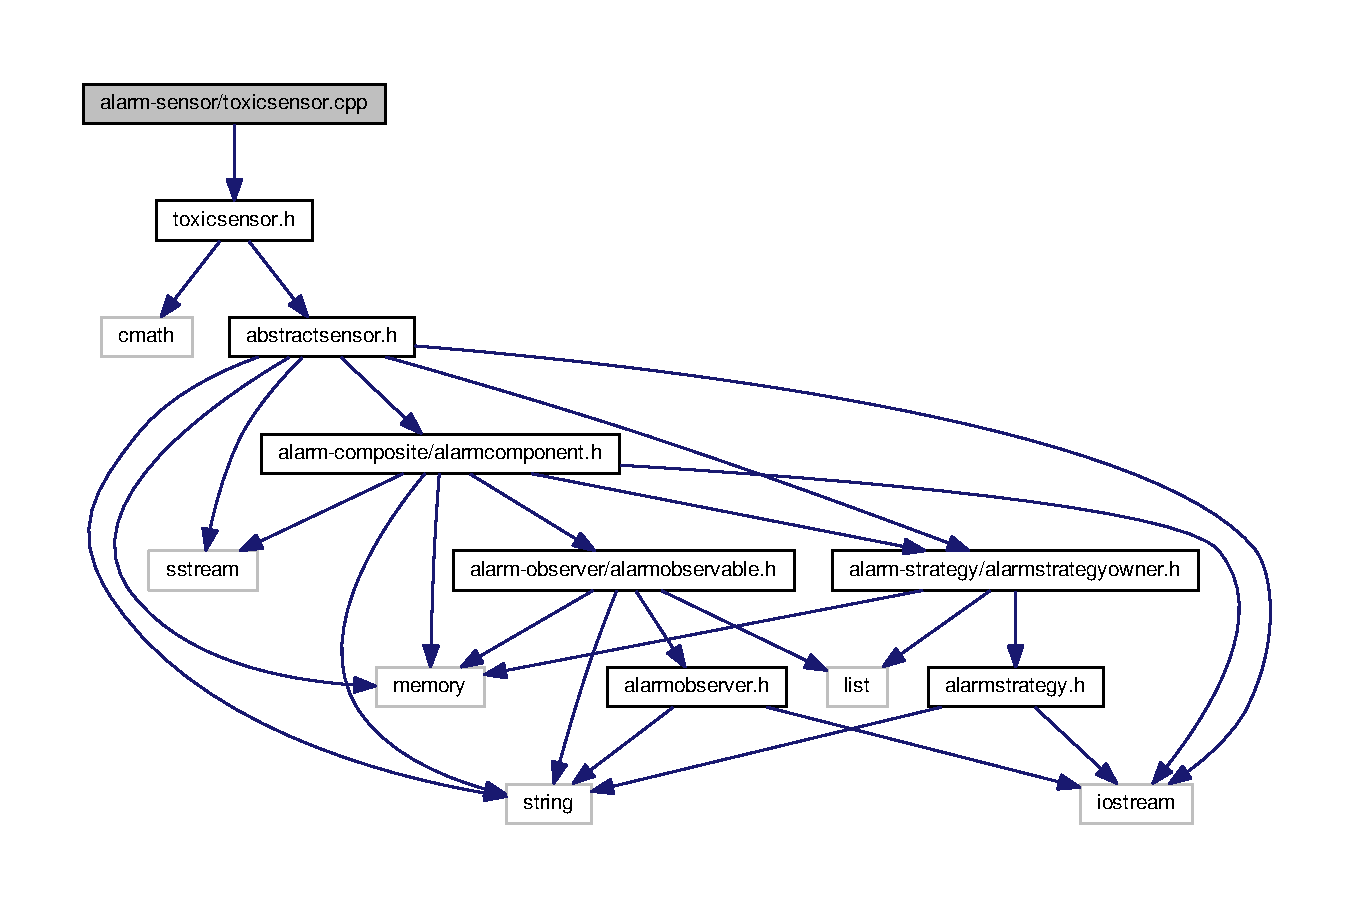
\includegraphics[width=350pt]{toxicsensor_8cpp__incl}
\end{center}
\end{figure}


\subsection{Detailed Description}
\hyperlink{classToxicSensor}{Toxic\+Sensor} class definition

\begin{DoxyVersion}{Version}
1.\+0
\end{DoxyVersion}
\begin{DoxyAuthor}{Author}
Vladimir Poliakov 

Brian Segers 
\end{DoxyAuthor}

\hypertarget{toxicsensor_8h}{}\section{alarm-\/sensor/toxicsensor.h File Reference}
\label{toxicsensor_8h}\index{alarm-\/sensor/toxicsensor.\+h@{alarm-\/sensor/toxicsensor.\+h}}
{\ttfamily \#include $<$cmath$>$}\\*
{\ttfamily \#include \char`\"{}abstractsensor.\+h\char`\"{}}\\*
Include dependency graph for toxicsensor.\+h\+:
\nopagebreak
\begin{figure}[H]
\begin{center}
\leavevmode
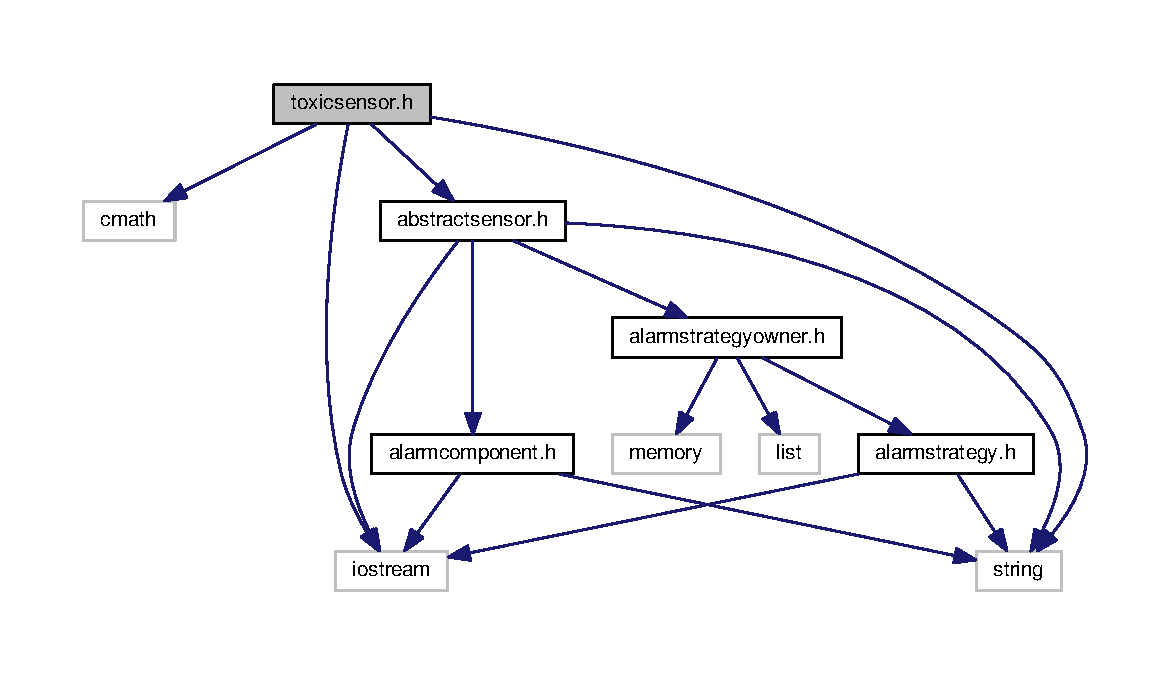
\includegraphics[width=350pt]{toxicsensor_8h__incl}
\end{center}
\end{figure}
\subsection*{Classes}
\begin{DoxyCompactItemize}
\item 
class \hyperlink{classToxicSensor}{Toxic\+Sensor}
\begin{DoxyCompactList}\small\item\em Toxic sensor class Dummy implementation of toxic sensor component. Intended for testing purposes. \end{DoxyCompactList}\end{DoxyCompactItemize}
\subsection*{Functions}
\begin{DoxyCompactItemize}
\item 
std\+::ostream \& \hyperlink{toxicsensor_8h_af572b22d42799f1737d02df351d8db04}{operator$<$$<$} (std\+::ostream \&lhs, const std\+::shared\+\_\+ptr$<$ \hyperlink{classToxicSensor}{Toxic\+Sensor} $>$ \&rhs)
\begin{DoxyCompactList}\small\item\em Passes info about the sensor to the output stream. \end{DoxyCompactList}\end{DoxyCompactItemize}


\subsection{Detailed Description}
\hyperlink{classToxicSensor}{Toxic\+Sensor} class declaration

\begin{DoxyVersion}{Version}
1.\+0
\end{DoxyVersion}
\begin{DoxyAuthor}{Author}
Vladimir Poliakov 

Brian Segers 
\end{DoxyAuthor}


\subsection{Function Documentation}
\index{toxicsensor.\+h@{toxicsensor.\+h}!operator$<$$<$@{operator$<$$<$}}
\index{operator$<$$<$@{operator$<$$<$}!toxicsensor.\+h@{toxicsensor.\+h}}
\subsubsection[{\texorpdfstring{operator$<$$<$(std\+::ostream \&lhs, const std\+::shared\+\_\+ptr$<$ Toxic\+Sensor $>$ \&rhs)}{operator<<(std::ostream &lhs, const std::shared_ptr< ToxicSensor > &rhs)}}]{\setlength{\rightskip}{0pt plus 5cm}std\+::ostream\& operator$<$$<$ (
\begin{DoxyParamCaption}
\item[{std\+::ostream \&}]{lhs, }
\item[{const std\+::shared\+\_\+ptr$<$ {\bf Toxic\+Sensor} $>$ \&}]{rhs}
\end{DoxyParamCaption}
)\hspace{0.3cm}{\ttfamily [inline]}}\hypertarget{toxicsensor_8h_af572b22d42799f1737d02df351d8db04}{}\label{toxicsensor_8h_af572b22d42799f1737d02df351d8db04}


Passes info about the sensor to the output stream. 

\begin{DoxyNote}{Note}
This is an overloaded function 
\end{DoxyNote}

\hypertarget{alarmsignal_8cpp}{}\section{alarm-\/strategy/alarmsignal.cpp File Reference}
\label{alarmsignal_8cpp}\index{alarm-\/strategy/alarmsignal.\+cpp@{alarm-\/strategy/alarmsignal.\+cpp}}
{\ttfamily \#include \char`\"{}alarmsignal.\+h\char`\"{}}\\*
Include dependency graph for alarmsignal.\+cpp\+:\nopagebreak
\begin{figure}[H]
\begin{center}
\leavevmode
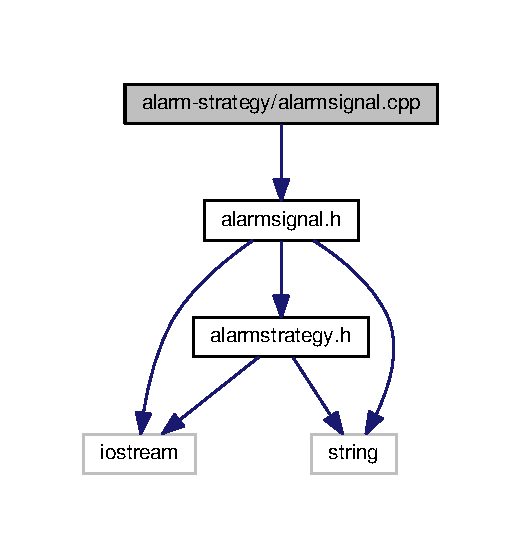
\includegraphics[width=250pt]{alarmsignal_8cpp__incl}
\end{center}
\end{figure}


\subsection{Detailed Description}
\hyperlink{classAlarmSignal}{Alarm\+Signal} class definition

\begin{DoxyVersion}{Version}
1.\+0
\end{DoxyVersion}
\begin{DoxyAuthor}{Author}
Vladimir Poliakov 

Brian Segers 
\end{DoxyAuthor}

\hypertarget{alarmsignal_8h}{}\section{alarm-\/strategy/alarmsignal.h File Reference}
\label{alarmsignal_8h}\index{alarm-\/strategy/alarmsignal.\+h@{alarm-\/strategy/alarmsignal.\+h}}
{\ttfamily \#include $<$iostream$>$}\\*
{\ttfamily \#include $<$string$>$}\\*
{\ttfamily \#include \char`\"{}alarmstrategy.\+h\char`\"{}}\\*
Include dependency graph for alarmsignal.\+h\+:\nopagebreak
\begin{figure}[H]
\begin{center}
\leavevmode
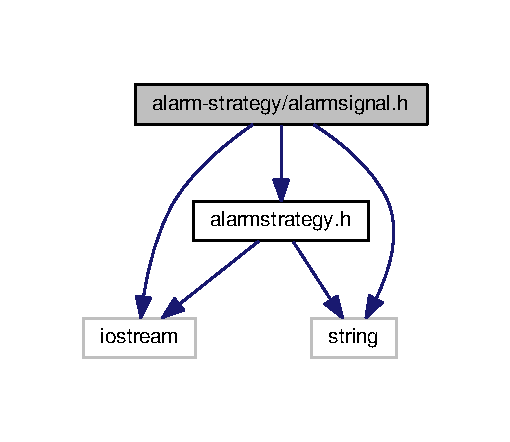
\includegraphics[width=245pt]{alarmsignal_8h__incl}
\end{center}
\end{figure}
This graph shows which files directly or indirectly include this file\+:\nopagebreak
\begin{figure}[H]
\begin{center}
\leavevmode
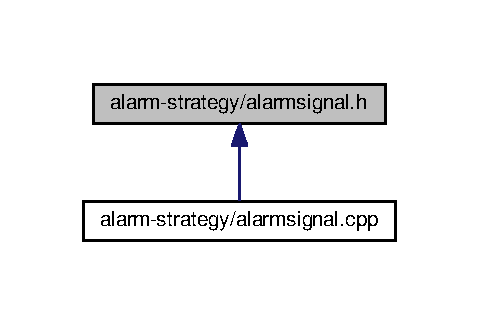
\includegraphics[width=230pt]{alarmsignal_8h__dep__incl}
\end{center}
\end{figure}
\subsection*{Classes}
\begin{DoxyCompactItemize}
\item 
class \hyperlink{classAlarmSignal}{Alarm\+Signal}
\begin{DoxyCompactList}\small\item\em Call police strategy class. \end{DoxyCompactList}\end{DoxyCompactItemize}


\subsection{Detailed Description}
\hyperlink{classAlarmSignal}{Alarm\+Signal} class declaration

\begin{DoxyVersion}{Version}
1.\+0
\end{DoxyVersion}
\begin{DoxyAuthor}{Author}
Vladimir Poliakov 

Brian Segers 
\end{DoxyAuthor}

\hypertarget{alarmstrategy_8cpp}{}\section{alarm-\/strategy/alarmstrategy.cpp File Reference}
\label{alarmstrategy_8cpp}\index{alarm-\/strategy/alarmstrategy.\+cpp@{alarm-\/strategy/alarmstrategy.\+cpp}}
{\ttfamily \#include \char`\"{}alarmstrategy.\+h\char`\"{}}\\*
Include dependency graph for alarmstrategy.\+cpp\+:\nopagebreak
\begin{figure}[H]
\begin{center}
\leavevmode
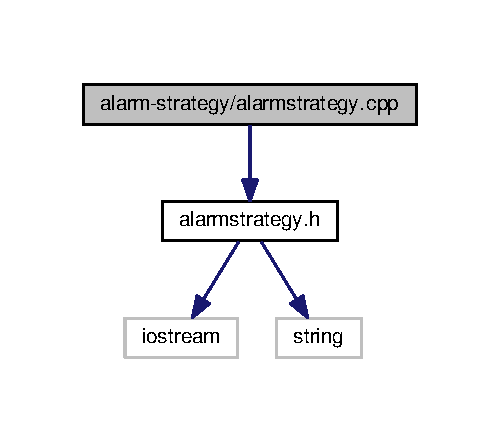
\includegraphics[width=240pt]{alarmstrategy_8cpp__incl}
\end{center}
\end{figure}


\subsection{Detailed Description}
\hyperlink{classAlarmStrategy}{Alarm\+Strategy} class definition

\begin{DoxyVersion}{Version}
1.\+0
\end{DoxyVersion}
\begin{DoxyAuthor}{Author}
Vladimir Poliakov 

Brian Segers 
\end{DoxyAuthor}

\hypertarget{alarmstrategy_8h}{}\section{alarmstrategy.\+h File Reference}
\label{alarmstrategy_8h}\index{alarmstrategy.\+h@{alarmstrategy.\+h}}
{\ttfamily \#include $<$iostream$>$}\\*
{\ttfamily \#include $<$string$>$}\\*
Include dependency graph for alarmstrategy.\+h\+:\nopagebreak
\begin{figure}[H]
\begin{center}
\leavevmode
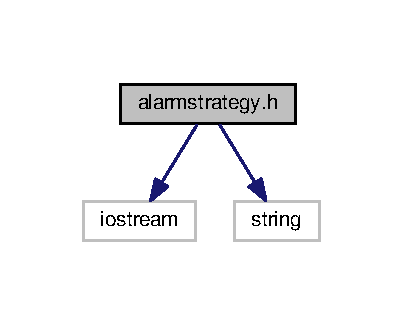
\includegraphics[width=194pt]{alarmstrategy_8h__incl}
\end{center}
\end{figure}
This graph shows which files directly or indirectly include this file\+:\nopagebreak
\begin{figure}[H]
\begin{center}
\leavevmode
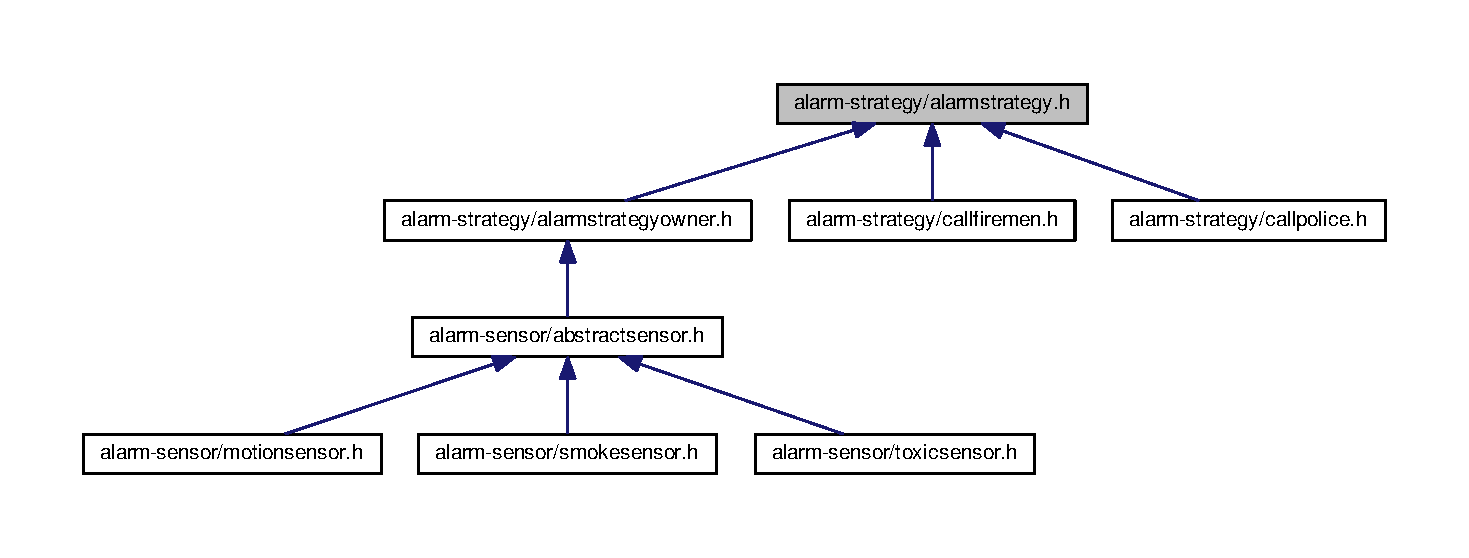
\includegraphics[width=350pt]{alarmstrategy_8h__dep__incl}
\end{center}
\end{figure}
\subsection*{Classes}
\begin{DoxyCompactItemize}
\item 
class \hyperlink{classAlarmStrategy}{Alarm\+Strategy}
\begin{DoxyCompactList}\small\item\em Strategy class implementation of strategy pattern. \end{DoxyCompactList}\end{DoxyCompactItemize}


\subsection{Detailed Description}
\hyperlink{classAlarmStrategy}{Alarm\+Strategy} class declaration

\begin{DoxyVersion}{Version}
1.\+0
\end{DoxyVersion}
\begin{DoxyAuthor}{Author}
Vladimir Poliakov 

Brian Segers 
\end{DoxyAuthor}

\hypertarget{alarmstrategyowner_8cpp}{}\section{alarm-\/strategy/alarmstrategyowner.cpp File Reference}
\label{alarmstrategyowner_8cpp}\index{alarm-\/strategy/alarmstrategyowner.\+cpp@{alarm-\/strategy/alarmstrategyowner.\+cpp}}
{\ttfamily \#include \char`\"{}alarmstrategyowner.\+h\char`\"{}}\\*
Include dependency graph for alarmstrategyowner.\+cpp\+:\nopagebreak
\begin{figure}[H]
\begin{center}
\leavevmode
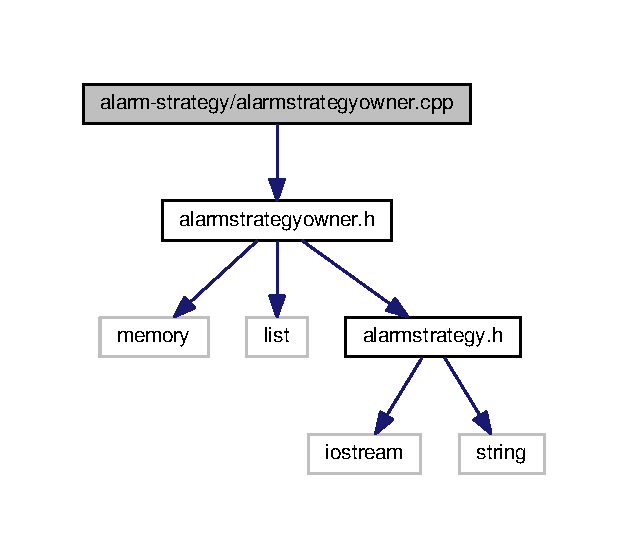
\includegraphics[width=302pt]{alarmstrategyowner_8cpp__incl}
\end{center}
\end{figure}


\subsection{Detailed Description}
\hyperlink{classAlarmStrategyOwner}{Alarm\+Strategy\+Owner} class definition

\begin{DoxyVersion}{Version}
1.\+0
\end{DoxyVersion}
\begin{DoxyAuthor}{Author}
Vladimir Poliakov 

Brian Segers 
\end{DoxyAuthor}

\hypertarget{alarmstrategyowner_8h}{}\section{alarm-\/strategy/alarmstrategyowner.h File Reference}
\label{alarmstrategyowner_8h}\index{alarm-\/strategy/alarmstrategyowner.\+h@{alarm-\/strategy/alarmstrategyowner.\+h}}
{\ttfamily \#include $<$memory$>$}\\*
{\ttfamily \#include $<$list$>$}\\*
{\ttfamily \#include \char`\"{}alarmstrategy.\+h\char`\"{}}\\*
Include dependency graph for alarmstrategyowner.\+h\+:
\nopagebreak
\begin{figure}[H]
\begin{center}
\leavevmode
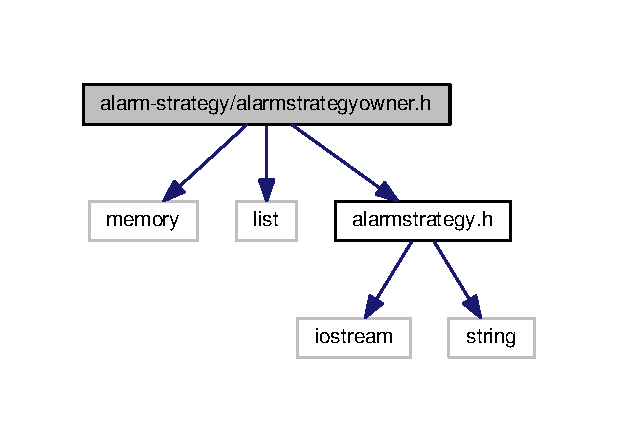
\includegraphics[width=297pt]{alarmstrategyowner_8h__incl}
\end{center}
\end{figure}
This graph shows which files directly or indirectly include this file\+:
\nopagebreak
\begin{figure}[H]
\begin{center}
\leavevmode
\includegraphics[width=350pt]{alarmstrategyowner_8h__dep__incl}
\end{center}
\end{figure}
\subsection*{Classes}
\begin{DoxyCompactItemize}
\item 
class \hyperlink{classAlarmStrategyOwner}{Alarm\+Strategy\+Owner}
\begin{DoxyCompactList}\small\item\em Context class implementation of strategy pattern. \end{DoxyCompactList}\end{DoxyCompactItemize}


\subsection{Detailed Description}
\hyperlink{classAlarmStrategyOwner}{Alarm\+Strategy\+Owner} class declaration

\begin{DoxyVersion}{Version}
1.\+0
\end{DoxyVersion}
\begin{DoxyAuthor}{Author}
Vladimir Poliakov 

Brian Segers 
\end{DoxyAuthor}

\hypertarget{waterdispenser_8cpp}{}\section{alarm-\/strategy/waterdispenser.cpp File Reference}
\label{waterdispenser_8cpp}\index{alarm-\/strategy/waterdispenser.\+cpp@{alarm-\/strategy/waterdispenser.\+cpp}}
{\ttfamily \#include \char`\"{}waterdispenser.\+h\char`\"{}}\\*
Include dependency graph for waterdispenser.\+cpp\+:\nopagebreak
\begin{figure}[H]
\begin{center}
\leavevmode
\includegraphics[width=259pt]{waterdispenser_8cpp__incl}
\end{center}
\end{figure}


\subsection{Detailed Description}
\hyperlink{classWaterDispenser}{Water\+Dispenser} class definition

\begin{DoxyVersion}{Version}
1.\+0
\end{DoxyVersion}
\begin{DoxyAuthor}{Author}
Vladimir Poliakov 

Brian Segers 
\end{DoxyAuthor}

\hypertarget{waterdispenser_8h}{}\section{alarm-\/strategy/waterdispenser.h File Reference}
\label{waterdispenser_8h}\index{alarm-\/strategy/waterdispenser.\+h@{alarm-\/strategy/waterdispenser.\+h}}
{\ttfamily \#include $<$iostream$>$}\\*
{\ttfamily \#include $<$string$>$}\\*
{\ttfamily \#include \char`\"{}alarmstrategy.\+h\char`\"{}}\\*
Include dependency graph for waterdispenser.\+h\+:\nopagebreak
\begin{figure}[H]
\begin{center}
\leavevmode
\includegraphics[width=253pt]{waterdispenser_8h__incl}
\end{center}
\end{figure}
This graph shows which files directly or indirectly include this file\+:\nopagebreak
\begin{figure}[H]
\begin{center}
\leavevmode
\includegraphics[width=247pt]{waterdispenser_8h__dep__incl}
\end{center}
\end{figure}
\subsection*{Classes}
\begin{DoxyCompactItemize}
\item 
class \hyperlink{classWaterDispenser}{Water\+Dispenser}
\begin{DoxyCompactList}\small\item\em Call firemen strategy class. \end{DoxyCompactList}\end{DoxyCompactItemize}


\subsection{Detailed Description}
\hyperlink{classWaterDispenser}{Water\+Dispenser} class declaration

\begin{DoxyVersion}{Version}
1.\+0
\end{DoxyVersion}
\begin{DoxyAuthor}{Author}
Vladimir Poliakov 

Brian Segers 
\end{DoxyAuthor}

%--- End generated contents ---

% Index
\backmatter
\newpage
\phantomsection
\clearemptydoublepage
\addcontentsline{toc}{chapter}{Index}
\printindex

\end{document}
